% Created 2016-02-07 Sun 17:48
\documentclass[number, sort&compress, review, 12pt]{elsarticle}
  \usepackage[utf8]{inputenc}
\usepackage{fixltx2e}
\usepackage{url}
\usepackage[version=3]{mhchem}
\usepackage{graphicx}
\usepackage{color}
\usepackage{amsmath}
\usepackage{textcomp}
\usepackage{wasysym}
\usepackage{latexsym}
\usepackage{amssymb}
\usepackage[linktocpage,
pdfstartview=FitH,
colorlinks,
linkcolor=blue,
anchorcolor=blue,
citecolor=blue,
filecolor=blue,
menucolor=blue,
urlcolor=blue]{hyperref}
\usepackage{attachfile}
\usepackage{longtable}
\usepackage{minted}
\usemintedstyle{emacs}
\newminted{python}{fontsize=\footnotesize}
\date{\today}
\title{supporting-information}
\begin{document}

\begin{frontmatter}
\title{Core-level shifts in Cu-Pd alloys as a function of bulk composition and structure}

\author[cmu]{Jacob Boes}
\author[cmu]{Peter Kondratyuk}
\author[cmu]{Chunrong Yin}
\author[cmu]{James B. Miller}
\author[cmu]{Andrew J. Gellman}
\author[cmu]{John R. Kitchin\corref{cor}}
\ead{jkitchin@andrew.cmu.edu}

\address[cmu]{Department of Chemical Engineering, Carnegie Mellon University, Pittsburgh, PA 15213}

\cortext[cor]{Corresponding author}
\end{frontmatter}

\tableofcontents

\section{Introduction}
\label{sec-1}
This document contains supporting data for the work, "Core-level shifts in Cu-Pd alloys as a function of bulk composition and structure." To make our work transparent and reproducible, we have stored most of the data used in this work in the JSON data format (\url{http://www.json.org}). The remaining data can be found in the tables at the end of this paper. The JSON file can be found here:

\attachfile{data.json}{(double-click to open)}.

JSON is a human-readable, language-independent data format. Code for parsing and generating JSON data is readily available in a large variety of programming languages including C, C++, Java, Python, Perl, etc\ldots{} We have used Python to read and write JSON data for all the examples below. Data inside the JSON file can also be viewed using online resources such as the viewer found here: \url{http://www.jsoneditoronline.org/}. Although there are many ways to interface with the data stored in the JSON file, we utilize the ASE database tool specifically designed for storing information about atoms objects. Further documentation on the ASE database and its features can be found here: \url{https://wiki.fysik.dtu.dk/ase/ase/db/db.html}. We organize information from the VASP calculations using descriptive keywords, which define the purpose of each calculation. A full list of the keywords used to categorize each calculation can be found in the code block below. Examples of how data is pulled from the database using this tool can be seen throughout the rest of the supporting information file.

\begin{minted}[frame=lines,fontsize=\scriptsize,linenos]{python}
from ase.db import connect
from textwrap import fill
db = connect('data.json')

# Select all entries in the ASE database.
entries = db.select()

for entry in entries:
    print entry.keywords

#all_keywords = []
#for entry in entries:
#    all_keywords.extend(entry.keywords)

# print fill('\n'.join(set(all_keywords)))
\end{minted}

\begin{verbatim}
[u'fcc', u'GS', u'72atom', u'1cl', u'0.88Cu']
[u'fcc', u'GS', u'72atom', u'1cl', u'0.75Cu']
[u'fcc', u'GS', u'72atom', u'1cl', u'0.62Cu']
[u'fcc', u'GS', u'72atom', u'1cl', u'0.50Cu']
[u'fcc', u'GS', u'72atom', u'1cl', u'0.38Cu']
[u'fcc', u'GS', u'72atom', u'1cl', u'0.25Cu']
[u'fcc', u'GS', u'72atom', u'1cl', u'0.17Cu']
[u'fcc', u'GS', u'72atom', u'1cl', u'1.00Cu']
[u'fcc', u'GS', u'72atom', u'0cl', u'1.00Cu']
[u'fcc', u'GS', u'72atom', u'0cl', u'0.88Cu']
[u'fcc', u'GS', u'72atom', u'0cl', u'0.75Cu']
[u'fcc', u'GS', u'72atom', u'0cl', u'0.62Cu']
[u'fcc', u'GS', u'72atom', u'0cl', u'0.50Cu']
[u'fcc', u'GS', u'72atom', u'0cl', u'0.38Cu']
[u'fcc', u'GS', u'72atom', u'0cl', u'0.25Cu']
[u'fcc', u'GS', u'72atom', u'0cl', u'0.17Cu']
[u'fcc', u'GS', u'72atom', u'0cl', u'0.00Cu']
[u'fcc', u'GS', u'24atom', u'1cl', u'1.00Cu']
[u'fcc', u'GS', u'24atom', u'1cl', u'0.50Cu']
[u'fcc', u'GS', u'24atom', u'1cl', u'0.75Cu']
[u'fcc', u'GS', u'24atom', u'1cl', u'0.25Cu']
[u'fcc', u'GS', u'24atom', u'1cl', u'0.17Cu']
[u'fcc', u'GS', u'24atom', u'1cl', u'0.62Cu']
[u'fcc', u'GS', u'24atom', u'1cl', u'0.88Cu']
[u'fcc', u'GS', u'24atom', u'1cl', u'0.38Cu']
[u'fcc', u'GS', u'24atom', u'0cl', u'1.00Cu']
[u'fcc', u'GS', u'24atom', u'0cl', u'0.00Cu']
[u'fcc', u'GS', u'24atom', u'0cl', u'0.75Cu']
[u'fcc', u'GS', u'24atom', u'0cl', u'0.25Cu']
[u'fcc', u'GS', u'24atom', u'0cl', u'0.50Cu']
[u'fcc', u'GS', u'24atom', u'0cl', u'0.62Cu']
[u'fcc', u'GS', u'24atom', u'0cl', u'0.88Cu']
[u'fcc', u'GS', u'24atom', u'0cl', u'0.38Cu']
[u'fcc', u'GS', u'24atom', u'0cl', u'0.17Cu']
[u'fcc', u'GS', u'54atom', u'0.50lat', u'ensam', u'I0C0', u'0cl']
[u'fcc', u'GS', u'54atom', u'0.50lat', u'ensam', u'I0C0', u'1cl']
[u'fcc', u'GS', u'54atom', u'0.50lat', u'ensam', u'I1C0', u'0cl']
[u'fcc', u'GS', u'54atom', u'0.50lat', u'ensam', u'I1C0', u'1cl']
[u'fcc', u'GS', u'54atom', u'0.50lat', u'ensam', u'I2C0', u'0cl']
[u'fcc', u'GS', u'54atom', u'0.50lat', u'ensam', u'I2C0', u'1cl']
[u'fcc', u'GS', u'54atom', u'0.50lat', u'ensam', u'I2C1', u'0cl']
[u'fcc', u'GS', u'54atom', u'0.50lat', u'ensam', u'I2C1', u'1cl']
[u'fcc', u'GS', u'54atom', u'0.50lat', u'ensam', u'I2C2', u'0cl']
[u'fcc', u'GS', u'54atom', u'0.50lat', u'ensam', u'I2C2', u'1cl']
[u'fcc', u'GS', u'54atom', u'0.50lat', u'ensam', u'I3C0', u'0cl']
[u'fcc', u'GS', u'54atom', u'0.50lat', u'ensam', u'I3C0', u'1cl']
[u'fcc', u'GS', u'54atom', u'0.50lat', u'ensam', u'I3C1', u'0cl']
[u'fcc', u'GS', u'54atom', u'0.50lat', u'ensam', u'I3C1', u'1cl']
[u'fcc', u'GS', u'54atom', u'0.50lat', u'ensam', u'I3C2', u'0cl']
[u'fcc', u'GS', u'54atom', u'0.50lat', u'ensam', u'I3C2', u'1cl']
[u'fcc', u'GS', u'54atom', u'0.50lat', u'ensam', u'I4C0', u'0cl']
[u'fcc', u'GS', u'54atom', u'0.50lat', u'ensam', u'I4C0', u'1cl']
[u'fcc', u'GS', u'54atom', u'0.50lat', u'ensam', u'I4C1', u'0cl']
[u'fcc', u'GS', u'54atom', u'0.50lat', u'ensam', u'I4C1', u'1cl']
[u'fcc', u'GS', u'54atom', u'0.50lat', u'ensam', u'I4C2', u'0cl']
[u'fcc', u'GS', u'54atom', u'0.50lat', u'ensam', u'I4C2', u'1cl']
[u'fcc', u'GS', u'54atom', u'0.50lat', u'ensam', u'I4C3', u'0cl']
[u'fcc', u'GS', u'54atom', u'0.50lat', u'ensam', u'I4C3', u'1cl']
[u'fcc', u'GS', u'54atom', u'0.50lat', u'ensam', u'I4C4', u'0cl']
[u'fcc', u'GS', u'54atom', u'0.50lat', u'ensam', u'I4C4', u'1cl']
[u'fcc', u'GS', u'54atom', u'0.50lat', u'ensam', u'I5C0', u'0cl']
[u'fcc', u'GS', u'54atom', u'0.50lat', u'ensam', u'I5C0', u'1cl']
[u'fcc', u'GS', u'54atom', u'0.50lat', u'ensam', u'I5C1', u'0cl']
[u'fcc', u'GS', u'54atom', u'0.50lat', u'ensam', u'I5C1', u'1cl']
[u'fcc', u'GS', u'54atom', u'0.50lat', u'ensam', u'I5C2', u'0cl']
[u'fcc', u'GS', u'54atom', u'0.50lat', u'ensam', u'I5C2', u'1cl']
[u'fcc', u'GS', u'54atom', u'0.50lat', u'dis', u'0cl', u'0']
[u'fcc', u'GS', u'54atom', u'0.50lat', u'dis', u'0cl', u'1']
[u'fcc', u'GS', u'54atom', u'0.50lat', u'dis', u'0cl', u'2']
[u'fcc', u'GS', u'54atom', u'0.50lat', u'dis', u'0cl', u'3']
[u'fcc', u'GS', u'54atom', u'0.50lat', u'dis', u'0cl', u'4']
[u'fcc', u'GS', u'54atom', u'0.50lat', u'dis', u'0cl', u'5']
[u'fcc', u'GS', u'54atom', u'0.50lat', u'dis', u'1cl', u'0']
[u'fcc', u'GS', u'54atom', u'0.50lat', u'dis', u'1cl', u'1']
[u'fcc', u'GS', u'54atom', u'0.50lat', u'dis', u'1cl', u'2']
[u'fcc', u'GS', u'54atom', u'0.50lat', u'dis', u'1cl', u'3']
[u'fcc', u'GS', u'54atom', u'0.50lat', u'dis', u'1cl', u'4']
[u'fcc', u'GS', u'54atom', u'0.50lat', u'dis', u'1cl', u'5']
[u'fcc', u'RN', u'64atom', u'1cl', u'0.88Cu']
[u'fcc', u'RN', u'64atom', u'1cl', u'0.75Cu']
[u'fcc', u'RN', u'64atom', u'1cl', u'0.62Cu']
[u'fcc', u'RN', u'64atom', u'1cl', u'0.50Cu']
[u'fcc', u'RN', u'64atom', u'1cl', u'0.38Cu']
[u'fcc', u'RN', u'64atom', u'1cl', u'0.25Cu']
[u'fcc', u'RN', u'64atom', u'1cl', u'0.12Cu']
[u'fcc', u'RN', u'64atom', u'1cl', u'1.00Cu']
[u'fcc', u'RN', u'64atom', u'1cl', u'0.50Cu-wid', u'32']
[u'fcc', u'RN', u'64atom', u'1cl', u'0.50Cu-wid', u'33']
[u'fcc', u'RN', u'64atom', u'1cl', u'0.50Cu-wid', u'34']
[u'fcc', u'RN', u'64atom', u'1cl', u'0.50Cu-wid', u'35']
[u'fcc', u'RN', u'64atom', u'1cl', u'0.50Cu-wid', u'36']
[u'fcc', u'RN', u'64atom', u'1cl', u'0.50Cu-wid', u'37']
[u'fcc', u'RN', u'64atom', u'1cl', u'0.50Cu-wid', u'38']
[u'fcc', u'RN', u'64atom', u'1cl', u'0.50Cu-wid', u'39']
[u'fcc', u'RN', u'64atom', u'1cl', u'0.50Cu-wid', u'40']
[u'fcc', u'RN', u'64atom', u'1cl', u'0.50Cu-wid', u'41']
[u'fcc', u'RN', u'64atom', u'1cl', u'0.50Cu-wid', u'42']
[u'fcc', u'RN', u'64atom', u'1cl', u'0.50Cu-wid', u'43']
[u'fcc', u'RN', u'64atom', u'1cl', u'0.50Cu-wid', u'44']
[u'fcc', u'RN', u'64atom', u'1cl', u'0.50Cu-wid', u'45']
[u'fcc', u'RN', u'64atom', u'1cl', u'0.50Cu-wid', u'46']
[u'fcc', u'RN', u'64atom', u'1cl', u'0.50Cu-wid', u'47']
[u'fcc', u'RN', u'64atom', u'1cl', u'0.50Cu-wid', u'48']
[u'fcc', u'RN', u'64atom', u'1cl', u'0.50Cu-wid', u'49']
[u'fcc', u'RN', u'64atom', u'1cl', u'0.50Cu-wid', u'50']
[u'fcc', u'RN', u'64atom', u'1cl', u'0.50Cu-wid', u'51']
[u'fcc', u'RN', u'64atom', u'1cl', u'0.50Cu-wid', u'52']
[u'fcc', u'RN', u'64atom', u'1cl', u'0.50Cu-wid', u'53']
[u'fcc', u'RN', u'64atom', u'1cl', u'0.50Cu-wid', u'54']
[u'fcc', u'RN', u'64atom', u'1cl', u'0.50Cu-wid', u'55']
[u'fcc', u'RN', u'64atom', u'1cl', u'0.50Cu-wid', u'56']
[u'fcc', u'RN', u'64atom', u'1cl', u'0.50Cu-wid', u'57']
[u'fcc', u'RN', u'64atom', u'1cl', u'0.50Cu-wid', u'58']
[u'fcc', u'RN', u'64atom', u'1cl', u'0.50Cu-wid', u'59']
[u'fcc', u'RN', u'64atom', u'1cl', u'0.50Cu-wid', u'60']
[u'fcc', u'RN', u'64atom', u'1cl', u'0.50Cu-wid', u'61']
[u'fcc', u'RN', u'64atom', u'1cl', u'0.50Cu-wid', u'62']
[u'fcc', u'RN', u'64atom', u'1cl', u'0.50Cu-wid', u'63']
[u'fcc', u'RN', u'64atom', u'0cl', u'1.00Cu']
[u'fcc', u'RN', u'64atom', u'0cl', u'0.00Cu']
[u'fcc', u'RN', u'64atom', u'0cl', u'0.50Cu']
[u'fcc', u'RN', u'64atom', u'0cl', u'0.88Cu']
[u'fcc', u'RN', u'64atom', u'0cl', u'0.75Cu']
[u'fcc', u'RN', u'64atom', u'0cl', u'0.38Cu']
[u'fcc', u'RN', u'64atom', u'0cl', u'0.25Cu']
[u'fcc', u'RN', u'64atom', u'0cl', u'0.12Cu']
[u'fcc', u'RN', u'64atom', u'0cl', u'0.62Cu']
[u'bcc', u'GS', u'72atom', u'0.95frac', u'0cl', u'0.50Cu']
[u'bcc', u'GS', u'72atom', u'0.95frac', u'1cl', u'0.50Cu']
[u'bcc', u'GS', u'72atom', u'1.05frac', u'0cl', u'0.50Cu']
[u'bcc', u'GS', u'72atom', u'1.05frac', u'1cl', u'0.50Cu']
[u'bcc', u'GS', u'72atom', u'1.00frac', u'1cl', u'0.67Cu']
[u'bcc', u'GS', u'72atom', u'1.00frac', u'1cl', u'0.50Cu']
[u'bcc', u'GS', u'72atom', u'1.00frac', u'1cl', u'0.33Cu']
[u'bcc', u'GS', u'72atom', u'1.00frac', u'1cl', u'0.25Cu']
[u'bcc', u'GS', u'72atom', u'1.00frac', u'1cl', u'1.00Cu']
[u'bcc', u'GS', u'72atom', u'1.00frac', u'0cl', u'0.67Cu']
[u'bcc', u'GS', u'72atom', u'1.00frac', u'0cl', u'0.50Cu']
[u'bcc', u'GS', u'72atom', u'1.00frac', u'0cl', u'0.33Cu']
[u'bcc', u'GS', u'72atom', u'1.00frac', u'0cl', u'0.25Cu']
[u'bcc', u'GS', u'72atom', u'1.00frac', u'0cl', u'1.00Cu']
[u'bcc', u'GS', u'72atom', u'1.00frac', u'0cl', u'0.00Cu']
[u'bcc', u'GS', u'54atom', u'0.40lat', u'dis', u'0cl', u'0']
[u'bcc', u'GS', u'54atom', u'0.40lat', u'dis', u'0cl', u'1']
[u'bcc', u'GS', u'54atom', u'0.40lat', u'dis', u'0cl', u'2']
[u'bcc', u'GS', u'54atom', u'0.40lat', u'dis', u'0cl', u'3']
[u'bcc', u'GS', u'54atom', u'0.40lat', u'dis', u'0cl', u'4']
[u'bcc', u'GS', u'54atom', u'0.40lat', u'dis', u'1cl', u'0']
[u'bcc', u'GS', u'54atom', u'0.40lat', u'dis', u'1cl', u'1']
[u'bcc', u'GS', u'54atom', u'0.40lat', u'dis', u'1cl', u'2']
[u'bcc', u'GS', u'54atom', u'0.40lat', u'dis', u'1cl', u'3']
[u'bcc', u'GS', u'54atom', u'0.40lat', u'dis', u'1cl', u'4']
[u'bcc', u'GS', u'54atom', u'0.40lat', u'ensam', u'I2C0', u'0cl']
[u'bcc', u'GS', u'54atom', u'0.40lat', u'ensam', u'I2C0', u'1cl']
[u'bcc', u'GS', u'54atom', u'0.40lat', u'ensam', u'I2C1', u'0cl']
[u'bcc', u'GS', u'54atom', u'0.40lat', u'ensam', u'I2C1', u'1cl']
[u'bcc', u'GS', u'54atom', u'0.40lat', u'ensam', u'I2C2', u'0cl']
[u'bcc', u'GS', u'54atom', u'0.40lat', u'ensam', u'I2C2', u'1cl']
[u'bcc', u'GS', u'54atom', u'0.40lat', u'ensam', u'I3C0', u'0cl']
[u'bcc', u'GS', u'54atom', u'0.40lat', u'ensam', u'I3C0', u'1cl']
[u'bcc', u'GS', u'54atom', u'0.40lat', u'ensam', u'I3C1', u'0cl']
[u'bcc', u'GS', u'54atom', u'0.40lat', u'ensam', u'I3C1', u'1cl']
[u'bcc', u'GS', u'54atom', u'0.40lat', u'ensam', u'I3C2', u'0cl']
[u'bcc', u'GS', u'54atom', u'0.40lat', u'ensam', u'I3C2', u'1cl']
[u'bcc', u'GS', u'54atom', u'0.40lat', u'ensam', u'I4C0', u'0cl']
[u'bcc', u'GS', u'54atom', u'0.40lat', u'ensam', u'I4C0', u'1cl']
[u'bcc', u'GS', u'54atom', u'0.40lat', u'ensam', u'I4C1', u'0cl']
[u'bcc', u'GS', u'54atom', u'0.40lat', u'ensam', u'I4C1', u'1cl']
[u'bcc', u'GS', u'54atom', u'0.40lat', u'ensam', u'I4C2', u'0cl']
[u'bcc', u'GS', u'54atom', u'0.40lat', u'ensam', u'I4C2', u'1cl']
[u'bcc', u'GS', u'54atom', u'0.40lat', u'ensam', u'I4C3', u'0cl']
[u'bcc', u'GS', u'54atom', u'0.40lat', u'ensam', u'I4C3', u'1cl']
[u'bcc', u'GS', u'54atom', u'0.40lat', u'ensam', u'I4C4', u'0cl']
[u'bcc', u'GS', u'54atom', u'0.40lat', u'ensam', u'I4C4', u'1cl']
[u'bcc', u'GS', u'54atom', u'0.40lat', u'ensam', u'I5C0', u'0cl']
[u'bcc', u'GS', u'54atom', u'0.40lat', u'ensam', u'I5C0', u'1cl']
[u'bcc', u'GS', u'54atom', u'0.40lat', u'ensam', u'I5C1', u'0cl']
[u'bcc', u'GS', u'54atom', u'0.40lat', u'ensam', u'I5C1', u'1cl']
[u'bcc', u'GS', u'54atom', u'0.40lat', u'ensam', u'I5C2', u'0cl']
[u'bcc', u'GS', u'54atom', u'0.40lat', u'ensam', u'I5C2', u'1cl']
[u'bcc', u'GS', u'54atom', u'0.35lat', u'dis', u'0cl', u'0']
[u'bcc', u'GS', u'54atom', u'0.35lat', u'dis', u'1cl', u'0']
[u'bcc', u'GS', u'54atom', u'0.45lat', u'dis', u'0cl', u'0']
[u'bcc', u'GS', u'54atom', u'0.45lat', u'dis', u'1cl', u'0']
[u'bcc', u'GS', u'54atom', u'0.55lat', u'dis', u'0cl', u'0']
[u'bcc', u'GS', u'54atom', u'0.55lat', u'dis', u'1cl', u'0']
[u'bcc', u'GS', u'54atom', u'0.50lat', u'dis', u'0cl', u'0']
[u'bcc', u'GS', u'54atom', u'0.50lat', u'dis', u'1cl', u'0']
[u'bcc', u'RN', u'64atom', u'1cl', u'1.00Cu']
[u'bcc', u'RN', u'64atom', u'1cl', u'0.50Cu-wid', u'0']
[u'bcc', u'RN', u'64atom', u'1cl', u'0.50Cu-wid', u'33']
[u'bcc', u'RN', u'64atom', u'1cl', u'0.50Cu-wid', u'34']
[u'bcc', u'RN', u'64atom', u'1cl', u'0.50Cu-wid', u'35']
[u'bcc', u'RN', u'64atom', u'1cl', u'0.50Cu-wid', u'36']
[u'bcc', u'RN', u'64atom', u'1cl', u'0.50Cu-wid', u'37']
[u'bcc', u'RN', u'64atom', u'1cl', u'0.50Cu-wid', u'38']
[u'bcc', u'RN', u'64atom', u'1cl', u'0.50Cu-wid', u'39']
[u'bcc', u'RN', u'64atom', u'1cl', u'0.50Cu-wid', u'40']
[u'bcc', u'RN', u'64atom', u'1cl', u'0.50Cu-wid', u'41']
[u'bcc', u'RN', u'64atom', u'1cl', u'0.50Cu-wid', u'42']
[u'bcc', u'RN', u'64atom', u'1cl', u'0.50Cu-wid', u'43']
[u'bcc', u'RN', u'64atom', u'1cl', u'0.50Cu-wid', u'44']
[u'bcc', u'RN', u'64atom', u'1cl', u'0.50Cu-wid', u'45']
[u'bcc', u'RN', u'64atom', u'1cl', u'0.50Cu-wid', u'46']
[u'bcc', u'RN', u'64atom', u'1cl', u'0.50Cu-wid', u'47']
[u'bcc', u'RN', u'64atom', u'1cl', u'0.50Cu-wid', u'48']
[u'bcc', u'RN', u'64atom', u'1cl', u'0.50Cu-wid', u'49']
[u'bcc', u'RN', u'64atom', u'1cl', u'0.50Cu-wid', u'50']
[u'bcc', u'RN', u'64atom', u'1cl', u'0.50Cu-wid', u'51']
[u'bcc', u'RN', u'64atom', u'1cl', u'0.50Cu-wid', u'52']
[u'bcc', u'RN', u'64atom', u'1cl', u'0.50Cu-wid', u'53']
[u'bcc', u'RN', u'64atom', u'1cl', u'0.50Cu-wid', u'54']
[u'bcc', u'RN', u'64atom', u'1cl', u'0.50Cu-wid', u'55']
[u'bcc', u'RN', u'64atom', u'1cl', u'0.50Cu-wid', u'56']
[u'bcc', u'RN', u'64atom', u'1cl', u'0.50Cu-wid', u'57']
[u'bcc', u'RN', u'64atom', u'1cl', u'0.50Cu-wid', u'58']
[u'bcc', u'RN', u'64atom', u'1cl', u'0.50Cu-wid', u'59']
[u'bcc', u'RN', u'64atom', u'1cl', u'0.50Cu-wid', u'60']
[u'bcc', u'RN', u'64atom', u'1cl', u'0.50Cu-wid', u'61']
[u'bcc', u'RN', u'64atom', u'1cl', u'0.50Cu-wid', u'62']
[u'bcc', u'RN', u'64atom', u'1cl', u'0.50Cu-wid', u'63']
[u'bcc', u'RN', u'64atom', u'0cl', u'0.88Cu']
[u'bcc', u'RN', u'64atom', u'0cl', u'0.75Cu']
[u'bcc', u'RN', u'64atom', u'0cl', u'0.62Cu']
[u'bcc', u'RN', u'64atom', u'0cl', u'0.50Cu']
[u'bcc', u'RN', u'64atom', u'0cl', u'0.38Cu']
[u'bcc', u'RN', u'64atom', u'0cl', u'0.25Cu']
[u'bcc', u'RN', u'64atom', u'0cl', u'0.12Cu']
[u'bcc', u'RN', u'64atom', u'0cl', u'1.00Cu']
[u'bcc', u'RN', u'64atom', u'0cl', u'0.00Cu']
\end{verbatim}

\section{A Brief Note About the Supporting Information Document}
\label{sec-2}
The supporting information document was prepared in org-mode (\url{http://orgmode.org}) syntax, which was subsequently exported to \LaTeX{} and converted to a PDF. Briefly, org-mode is a plain text format that enables intermingling of text and code, with markup for typical document elements such as headings, links, tables, etc\ldots{}, and arbitrary inclusion of \LaTeX{} for equations. With the Emacs editor, the code in an org-mode document can be executed in place, and the output captured in the document. For example, tables can be generated by code, or the code for generating a figure can be embedded in the document. The data in tables can be used as input to other code blocks in the document as well. Org-mode enables selective export of the content to various formats including html, \LaTeX{}, and PDF. These features, and many others, make org-mode a convenient platform for reproducible research, where all of the steps leading to conclusions drawn in the work can be documented in one place, but where it may be desirable not to show all the details in every view. For example, in an exported manuscript where code should usually not be visible, or supporting information document such as this one where it is desirable to see the code. Nevertheless, it may still be valuable to go back to the source, for example, to figure out how some analysis was done, especially if all the code is not exported.

The org-mode source for this document can be found here: \attachfile{supporting-information.org}.

\section{Getting the Computational Details of a Calculation from the JSON file}
\label{sec-3}
Here is an example of opening the JSON file using the ASE database tool, and printing the calculation details for a single calculation. First we print all of the information stored and then show how specific information can be taken directly from the database, such as calculator INCAR parameters and total energy of the calculation.

\begin{minted}[frame=lines,fontsize=\scriptsize,linenos]{python}
from ase.db import connect
from textwrap import fill

db = connect('data.json')

# Select a specific entry in the database
example = db.select(['fcc', 'GS', '24atom', '0cl', '1.00Cu'])

# ASE database utilizes generator objects. To access the first,
# and only entry in this generator, we use '.next()'.
example = example.next()

# Here we print all of the information stored in the database
print fill(str(example)), '\n'

# Specific information can be pulled from the database by
# specifying the appropriate sub-dictionary name. This is
# shown for the INCAR parameters:
print 'The INCAR parameters:'
print fill(str(example.calculator_parameters.incar)), '\n'

# Here we print the total energy of the calculation:
print 'The total energy:'
print '{0} eV'.format(example.energy)
\end{minted}

\begin{verbatim}
{u'GS': 1, u'tags': array([0, 0, 0, 0, 0, 0, 0, 0, 0, 0, 0, 0, 0, 0,
0, 0, 0, 0, 0, 0, 0, 0, 0,        0]), u'energy': -89.298417,
u'calculator_parameters': {u'incar': {u'encut': 400.0, u'doc': u'INCAR
parameters', u'prec': u'Normal', u'nsim': 4, u'isif': 3, u'nbands':
160, u'ibrion': 2, u'lplane': True, u'ediffg': -0.02, u'ismear': 1,
u'ediff': 1e-06, u'npar': 4, u'nsw': 10}, u'doc': u'JSON
representation of a VASP calculation.\n\nenergy is in eV\nforces are
in eV/\\AA\nstress is in GPa (sxx, syy, szz,  syz, sxz, sxy)\nmagnetic
moments are in Bohr-magneton\nThe density of states is reported with
E_f at 0 eV.\nVolume is reported in \\AA^3\nCoordinates and cell
parameters are reported in \\AA\n\nIf atom-projected dos are included
they are in the form:\n{ados:{energy:data, {atom index: {orbital :
dos}}}\n', u'potcar': [[u'Cu', u'potpaw_PBE/Cu/POTCAR',
u'a44c591415026f53deb16a99ca3f06b1e69be10b']], u'input': {u'kpts':
array([3, 4, 7]), u'reciprocal': False, u'xc': u'PBE',
u'kpts_nintersections': None, u'setups': None, u'txt': u'-', u'gamma':
False}, u'atoms': {u'cell': array([[  7.27008008e+00,
3.42724757e-02,   7.35232202e+00],        [  5.44549051e+00,
5.39375647e+00,   3.30520765e-02],        [  5.58073992e-03,
3.61208260e+00,   3.68787361e+00]]), u'symbols': [u'Cu', u'Cu', u'Cu',
u'Cu', u'Cu', u'Cu', u'Cu', u'Cu', u'Cu', u'Cu', u'Cu', u'Cu', u'Cu',
u'Cu', u'Cu', u'Cu', u'Cu', u'Cu', u'Cu', u'Cu', u'Cu', u'Cu', u'Cu',
u'Cu'], u'tags': array([0, 0, 0, 0, 0, 0, 0, 0, 0, 0, 0, 0, 0, 0, 0,
0, 0, 0, 0, 0, 0, 0, 0,        0]), u'pbc': array([ True,  True,
True], dtype=bool), u'positions': array([[  0.00000000e+00,
0.00000000e+00,   0.00000000e+00],        [  2.79036996e-03,
1.80604130e+00,   1.84393680e+00],        [  1.81516350e+00,
1.79791882e+00,   1.10173588e-02],        [  1.81795387e+00,
3.60396012e+00,   1.85495416e+00],        [  3.63032700e+00,
3.59583765e+00,   2.20347177e-02],        [  3.63311737e+00,
5.40187894e+00,   1.86597152e+00],        [  1.81752002e+00,
8.56811893e-03,   1.83808050e+00],        [  1.82031039e+00,
1.81460942e+00,   3.68201731e+00],        [  3.63268352e+00,
1.80648694e+00,   1.84909786e+00],        [  3.63547389e+00,
3.61252824e+00,   3.69303467e+00],        [  5.44784702e+00,
3.60440576e+00,   1.86011522e+00],        [  5.45063739e+00,
5.41044706e+00,   3.70405203e+00],        [  3.63504004e+00,
1.71362379e-02,   3.67616101e+00],        [  3.63783041e+00,
1.82317754e+00,   5.52009781e+00],        [  5.45020354e+00,
1.81505506e+00,   3.68717837e+00],        [  5.45299391e+00,
3.62109636e+00,   5.53111517e+00],        [  7.26536704e+00,
3.61297388e+00,   3.69819573e+00],        [  7.26815741e+00,
5.41901518e+00,   5.54213253e+00],        [  5.45256006e+00,
2.57043568e-02,   5.51424151e+00],        [  5.45535043e+00,
1.83174565e+00,   7.35817832e+00],        [  7.26772356e+00,
1.82362318e+00,   5.52525887e+00],        [  7.27051393e+00,
3.62966448e+00,   7.36919568e+00],        [  9.08288706e+00,
3.62154200e+00,   5.53627623e+00],        [  9.08567743e+00,
5.42758330e+00,   7.38021303e+00]])}, u'data': {u'stress': array([
0.00044062,  0.00117381,  0.00037976,  0.00119491,  0.00035132,
-0.00011941]), u'doc': u'Data from the output of the calculation',
u'volume': 287.452162285601, u'total_energy': -89.298417, u'forces':
array([[ 0.,  0.,  0.],        [ 0.,  0.,  0.],        [ 0.,  0.,
0.],        [ 0.,  0.,  0.],        [ 0.,  0.,  0.],        [ 0.,  0.,
0.],        [ 0.,  0.,  0.],        [ 0.,  0.,  0.],        [ 0.,  0.,
0.],        [ 0.,  0.,  0.],        [ 0.,  0.,  0.],        [ 0.,  0.,
0.],        [ 0.,  0.,  0.],        [ 0.,  0.,  0.],        [ 0.,  0.,
0.],        [ 0.,  0.,  0.],        [ 0.,  0.,  0.],        [ 0.,  0.,
0.],        [ 0.,  0.,  0.],        [ 0.,  0.,  0.],        [ 0.,  0.,
0.],        [ 0.,  0.,  0.],        [ 0.,  0.,  0.],        [ 0.,  0.,
0.]]), u'fermi_level': 3.685}, u'metadata': {u'date.created':
1398438581.016546, u'uuid': u'a01f2baa-cc8b-11e3-b664-003048f5e49e',
u'date.created.ascii': u'Fri Apr 25 11:09:41 2014', u'user.username':
None, u'atoms.resort': array([ 0,  1,  2,  3,  4,  5,  6,  7,  8,  9,
10, 11, 12, 13, 14, 15, 16,        17, 18, 19, 20, 21, 22, 23]),
u'user.email': None, u'user.fullname': None, u'Cu.potential.git_hash':
u'a44c591415026f53deb16a99ca3f06b1e69be10b', u'atoms.tags': array([0,
0, 0, 0, 0, 0, 0, 0, 0, 0, 0, 0, 0, 0, 0, 0, 0, 0, 0, 0, 0, 0, 0,
0]), u'Cu.potential.path': u'potpaw_PBE/Cu/POTCAR'}}, u'fcc': 1,
u'numbers': array([29, 29, 29, 29, 29, 29, 29, 29, 29, 29, 29, 29, 29,
29, 29, 29, 29,        29, 29, 29, 29, 29, 29, 29]),
u'key_value_pairs': {u'GS': 1, u'_24atom': 1, u'_0cl': 1, u'fcc': 1,
u'_1_00Cu': 1}, u'mtime': 15.038292685183254, u'keywords': [u'fcc',
u'GS', u'24atom', u'0cl', u'1.00Cu'], u'_24atom': 1, u'_1_00Cu': 1,
'id': 26, u'ctime': 14.923533301677663, u'positions': array([[
0.00000000e+00,   0.00000000e+00,   0.00000000e+00],        [
2.79036996e-03,   1.80604130e+00,   1.84393680e+00],        [
1.81516350e+00,   1.79791882e+00,   1.10173588e-02],        [
1.81795387e+00,   3.60396012e+00,   1.85495416e+00],        [
3.63032700e+00,   3.59583765e+00,   2.20347177e-02],        [
3.63311737e+00,   5.40187894e+00,   1.86597152e+00],        [
1.81752002e+00,   8.56811893e-03,   1.83808050e+00],        [
1.82031039e+00,   1.81460942e+00,   3.68201731e+00],        [
3.63268352e+00,   1.80648694e+00,   1.84909786e+00],        [
3.63547389e+00,   3.61252824e+00,   3.69303467e+00],        [
5.44784702e+00,   3.60440576e+00,   1.86011522e+00],        [
5.45063739e+00,   5.41044706e+00,   3.70405203e+00],        [
3.63504004e+00,   1.71362379e-02,   3.67616101e+00],        [
3.63783041e+00,   1.82317754e+00,   5.52009781e+00],        [
5.45020354e+00,   1.81505506e+00,   3.68717837e+00],        [
5.45299391e+00,   3.62109636e+00,   5.53111517e+00],        [
7.26536704e+00,   3.61297388e+00,   3.69819573e+00],        [
7.26815741e+00,   5.41901518e+00,   5.54213253e+00],        [
5.45256006e+00,   2.57043568e-02,   5.51424151e+00],        [
5.45535043e+00,   1.83174565e+00,   7.35817832e+00],        [
7.26772356e+00,   1.82362318e+00,   5.52525887e+00],        [
7.27051393e+00,   3.62966448e+00,   7.36919568e+00],        [
9.08288706e+00,   3.62154200e+00,   5.53627623e+00],        [
9.08567743e+00,   5.42758330e+00,   7.38021303e+00]]), u'composition':
1.0, u'cell': array([[  7.27008008e+00,   3.42724757e-02,
7.35232202e+00],        [  5.44549051e+00,   5.39375647e+00,
3.30520765e-02],        [  5.58073992e-03,   3.61208260e+00,
3.68787361e+00]]), u'pbc': array([ True,  True,  True], dtype=bool),
u'_0cl': 1, u'calculator': u'vasp', u'unique_id':
u'f1a4a3c4f9a54c9878026ba21390287b', u'user': u'jboes'}

The INCAR parameters:
{u'nsw': 10, u'ediff': 1e-06, u'doc': u'INCAR parameters', u'encut':
400.0, u'nsim': 4, u'isif': 3, u'ibrion': 2, u'nbands': 160, u'prec':
u'Normal', u'ismear': 1, u'lplane': True, u'npar': 4, u'ediffg':
-0.02}

The total energy:
-89.298417 eV
\end{verbatim}

\section{Implementation of ICORELEVEL in VASP}
\label{sec-4}
Calculation of the CLS in VASP requires the use of the ICORELEVEL-tag. This section is designed to outline some of the possible functionalities of this tag and also has a few working examples. The documentation for the ICORELEVEL tag can be found on the VASP website: \url{http://cms.mpi.univie.ac.at/vasp/vasp/ICORELEVEL_tag_core_level_shifts.html}. This brief description makes reference to another article, Ref. \citenum{kohler-2004-densit-funct}, and references there in. Although these articles document the results of using the ICORELEVEL-tag, they do not provide specific details of the implementation.

ICORELEVEL has three setting: 0, 1, and 2. The default is 0 which runs the calculation normally. A setting of 1 will run the calculation normally, but at the end of each self consistent iteration the core level Eigen energies will be printed into the OUTCAR file. These values can be found quickly by performing a grep for 'the core state eigenenergies are'. The core-level Eigen energies are needed for CLS calculation methods other than complete screening (CS). Since the CS method only utilizes the total energy of a calculation, the 1 setting is not necessary for the purposes of this study.

The 2 setting will replace a number of core electrons from a species specified in the POSCAR/POTCAR file with a valence electron and then allow the valence electrons to relax. The remaining core electrons are not allowed to relax in VASP. The implications of this have not yet been fully explored. Specifying which electron will be removed is done using the CLNT-, CLN-, CLL-, and CLZ-tags. Details of these tags are included below.

\begin{itemize}
\item CLNT = The species. This an integer, N, which refers to Nth species in the POSCAR/POTCAR file. This species will need to be singled out in these input files which is discussed further in the examples provided below. NOTE: a value of 0 or 1 can be used to specify the first species in the POSCAR/POTCAR file.
\item CLN = The n quantum number of the excited core electron. i.e. for the 2p$_{\text{3/2}}$ electron, cln=2 (2nd shell electron)
\item CLL = the l quantum number of the excited core electron. i.e. for the 2p$_{\text{3/2}}$ electron, cll=1 (an electron in a p-orbital)
\item CLZ = electron count. This is a float, typically 0-1. Floats are allowed for implementation of the transition state method. For the second step in CS, a value of 1 is typical. A value of 0 is the same as icorelevel=1
\end{itemize}

For specific examples of how these calculations are implemented see the following code blocks:

\begin{minted}[frame=lines,fontsize=\scriptsize,linenos]{python}
from jasp import *

# This code demonstrates a standard DFT calculation using JASP
with jasp('CuPd/0cl',
          xc='PBE',            # Specify INCAR parameters
          encut=400,
          kpts=(8, 8, 8),
          ibrion=-1,
          ediff=1e-6,
          atoms=atoms) as calc:
    try:
        calc.calculate()
    except(VaspQueued, VaspSubmitted):
        pass

# This code shows the modifications to a standard JASP
# calculation to excite a core electron
with jasp('CuPd/1cl',
          xc='PBE',            # Specify INCAR parameters
          encut=400,
          kpts=(8, 8, 8),
          ibrion=-1,
          ediff=1e-6,
          setups={'0': 'Cu'},  # Create separate entry in POTCAR for atom index 0
          icorelevel=2,        # Perform core level shift calculation
          clnt=0,              # Excite atom index 0
          cln=2,               # 2p3/2 electorn for Cu core level shift
          cll=1,
          clz=1,
          atoms=atoms) as calc:
    try:
        calc.calculate()
    except(VaspQueued, VaspSubmitted):
        pass
\end{minted}

\section{Effects of ion-ion interaction}
\label{sec-5}
To gain some understanding of the effects caused by ion-ion interaction, 24 and 72 atom unit cells were created for similar compositions of relaxed ground state FCC CuPd compositions. A comparison of the core level shifts calculated for these structures are shown below in Figure \ref{fig-ion}. Comparison between these two structures shows up to 0.1 eV change in CLS energies of the 24 atom and 72 atom unit cell. This change is considered small on the overall trend observed.

\begin{figure}[H]
\centering
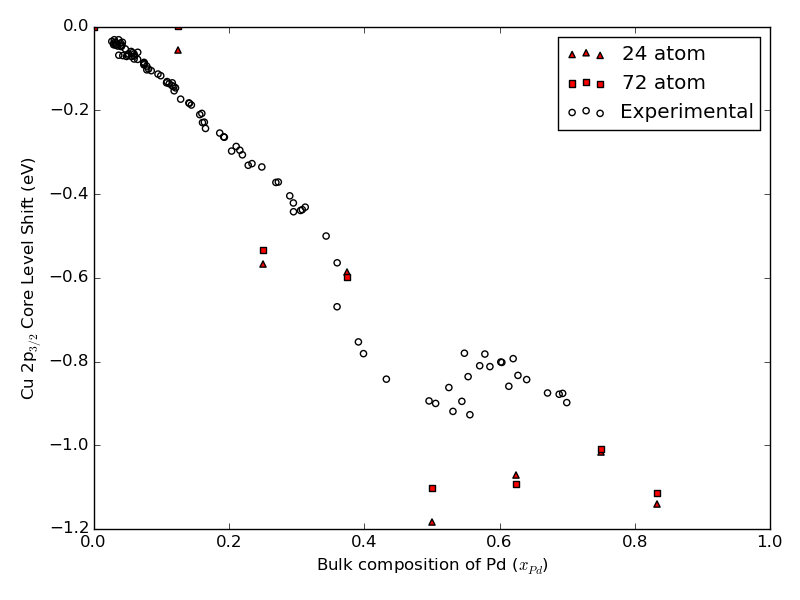
\includegraphics[width=4in]{./images/ion-int.png}
\caption{\label{fig-ion}Effects of ion-ion interaction between 24 and 72 atom super-cells for various identical structures of CuPd alloy. Computationally calculated Cu CLS (red) as compared to experimental results (black).}
\end{figure}

\begin{minted}[frame=lines,fontsize=\scriptsize,linenos]{python}
from ase.db import connect
import numpy as np
import matplotlib.pyplot as plt

# Import Gellman experimental data
d0x = np.array([entry[0] for entry in d0])
d0y = np.array([entry[1] for entry in d0])

# Loads the ASE database
db = connect('data.json')

# 24 atom unit cell
# Select reference energy of ground and ionized pure Cu
keys = ['fcc', 'GS', '24atom']

CLS24, COMP24 = [], []
for k in db.select(keys + ['1cl']):
    comp = k.keywords[-1]

    Cu0 = db.select(keys + ['0cl', '1.00Cu']).next().energy
    Cu1 = db.select(keys + ['1cl', '1.00Cu']).next().energy
    x0 = db.select(keys + ['0cl', comp]).next().energy
    x1 = k.energy

    cls0 = x0 - Cu0
    cls1 = x1 - Cu1

    COMP24.append(1.0 - k.composition)
    CLS24.append(cls1 - cls0)

# 72 atom unit cell
# Loads reference energy of ground and ionized pure Cu
keys = ['fcc', 'GS', '72atom']

CLS72, COMP72 = [], []
for k in db.select(keys + ['1cl']):
    comp = k.keywords[-1]

    Cu0 = db.select(keys + ['0cl', '1.00Cu']).next().energy
    Cu1 = db.select(keys + ['1cl', '1.00Cu']).next().energy
    x0 = db.select(keys + ['0cl', comp]).next().energy
    x1 = k.energy

    cls0 = x0 - Cu0
    cls1 = x1 - Cu1

    COMP72.append(1.0 - k.composition)
    CLS72.append(cls1 - cls0)

plt.figure()
plt.scatter(COMP24, CLS24, c='r', marker='^', label='24 atom')
plt.scatter(COMP72, CLS72, c='r', marker='s', label='72 atom')
plt.scatter(d0x, d0y, c='k', facecolor='none', label='Experimental')
plt.xlim(0, 1)
plt.xlabel('Bulk composition of Pd ($x_{Pd}$)')
plt.ylim(-1.2, 0.0)
plt.ylabel('Cu 2p$_{3/2}$ Core Level Shift (eV)')
plt.legend(loc='best')
plt.tight_layout()
plt.savefig('./images/ion-int.png')
\end{minted}

\section{CLS widening at 50 at.\% composition}
\label{sec-6}
It is well known that the local chemical environment can effect the CLS of an alloy. Since the method we use to calculate the CLS is based on the ionization of a single atom, the resulting CLS may not fully represent the averaged CLS in a random alloy. We demonstrate this effect below for the 50\% Pd composition of a randomly configured CuPd alloy. Figure \ref{fig-fccwid} shows a histogram of the Cu-shifts measured for 32 Cu atoms randomly ordered in a 64 atom fcc supercell, and Figure \ref{fig-bccwid} shows the same result in a 64 atom bcc supercell.

\begin{figure}[H]
\centering
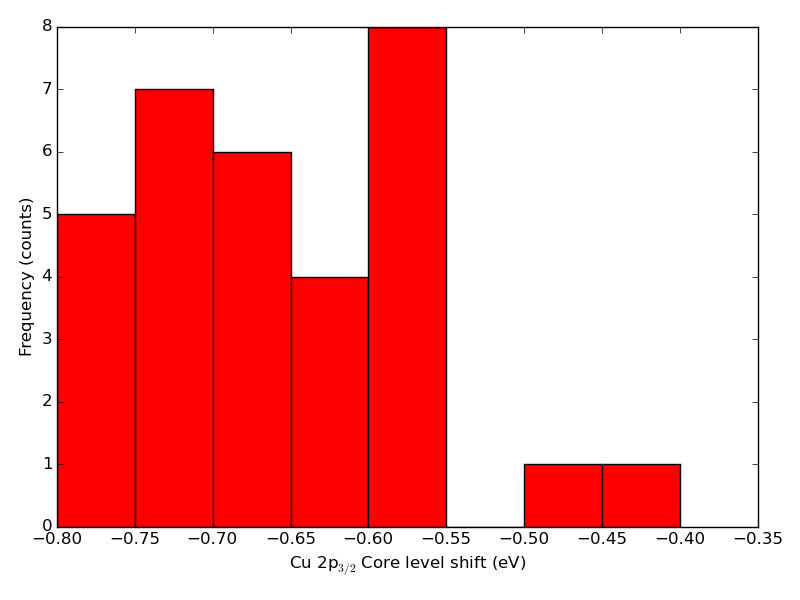
\includegraphics[width=4in]{./images/fcc-wid.png}
\caption{\label{fig-fccwid}Peak widening of 50\% Pd composition randomly configured bulk configuration of CuPd FCC alloy.}
\end{figure}
\begin{minted}[frame=lines,fontsize=\scriptsize,linenos]{python}
from ase.db import connect
import numpy as np
import matplotlib.pyplot as plt

# loads the ASE database and select certain keywords
db = connect('data.json')
keys = ['fcc', 'RN', '64atom']

CLS = []
for k in db.select(keys + ['1cl', '0.50Cu-wid']):
    Cu0 = db.select(keys + ['0cl', '1.00Cu']).next().energy
    Cu1 = db.select(keys + ['1cl', '1.00Cu']).next().energy
    x0 = db.select(keys + ['0cl', '0.50Cu']).next().energy
    x1 = k.energy

    cls0 = x0 - Cu0
    cls1 = x1 - Cu1

    CLS.append(cls1 - cls0)

CLS = np.array(CLS)

hist, bins = np.histogram(CLS, bins=8,
                          range=(round(min(CLS), 1),
                                 round(max(CLS), 1)))

width = 1 * (bins[1] - bins[0])
center = (bins[:-1] + bins[1:]) / 2
plt.bar(center, hist, align='center', width=width, color='r')

plt.xlabel('Cu 2p$_{3/2}$ Core level shift (eV)')
plt.ylabel('Frequency (counts)')
plt.tight_layout()

plt.savefig('images/fcc-wid.png')
\end{minted}


\begin{figure}[H]
\centering
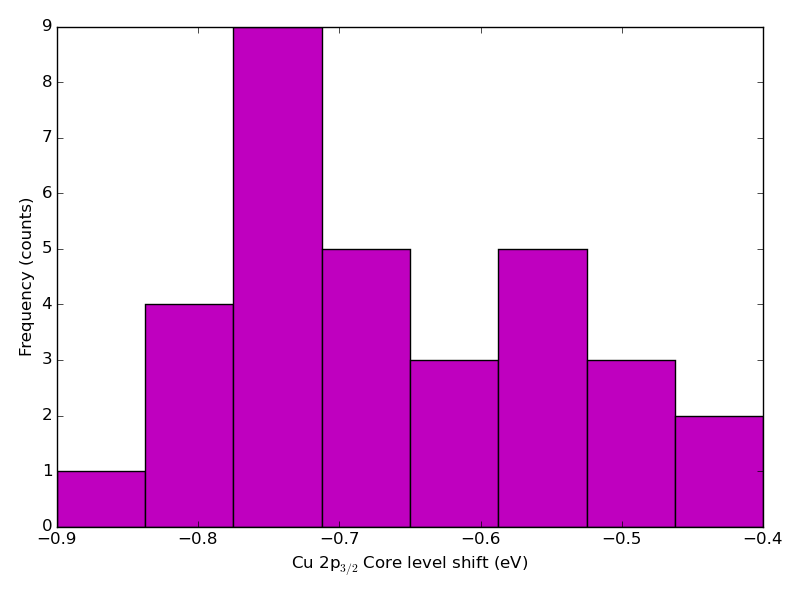
\includegraphics[width=4in]{./images/bcc-wid.png}
\caption{\label{fig-bccwid}Peak widening of 50\% Pd composition randomly configured bulk configuration of CuPd BCC alloy.}
\end{figure}

\begin{minted}[frame=lines,fontsize=\scriptsize,linenos]{python}
from ase.db import connect
import numpy as np
import matplotlib.pyplot as plt

# loads the ASE database and select certain keywords
db = connect('data.json')
keys = ['bcc', 'RN', '64atom']

CLS = []
for k in db.select(keys + ['1cl', '0.50Cu-wid']):
    Cu0 = db.select(keys + ['0cl', '1.00Cu']).next().energy
    Cu1 = db.select(keys + ['1cl', '1.00Cu']).next().energy
    x0 = db.select(keys + ['0cl', '0.50Cu']).next().energy
    x1 = k.energy

    cls0 = x0 - Cu0
    cls1 = x1 - Cu1

    CLS.append(cls1 - cls0)

CLS = np.array(CLS)

hist, bins = np.histogram(CLS, bins=8,
                          range=(round(min(CLS), 1),
                                 round(max(CLS), 1)))

width = 1 * (bins[1] - bins[0])
center = (bins[:-1] + bins[1:]) / 2
plt.bar(center, hist, align='center', width=width, color='m')

plt.xlabel('Cu 2p$_{3/2}$ Core level shift (eV)')
plt.ylabel('Frequency (counts)')
plt.tight_layout()

plt.savefig('images/bcc-wid.png')
\end{minted}

\section{Distinction between randomly ordered FCC and BCC}
\label{sec-7}
We have also performed a similar widening study on a randomly ordered BCC structure at 50\% Pd composition. These results are shown in Figure \ref{fig-bccwid}. Comparing Figures \ref{fig-fccwid} with \ref{fig-bccwid}, little difference is seen between the two distributions. This suggests that the effects of a change in structure on CLS energies are not nearly as important as those from atomic ordering.

We also see that there is a dramatic difference in the CLS seen in the B2 phase from the randomly configured alloy. There also appears the be relatively little difference between the Cu-shifts calculated between the ordered FCC and B2 phases. These results suggest that the compuational tools may not be able to easily distinguish between ordered phase types - only that an ordered phase exists.

\begin{figure}[H]
\centering
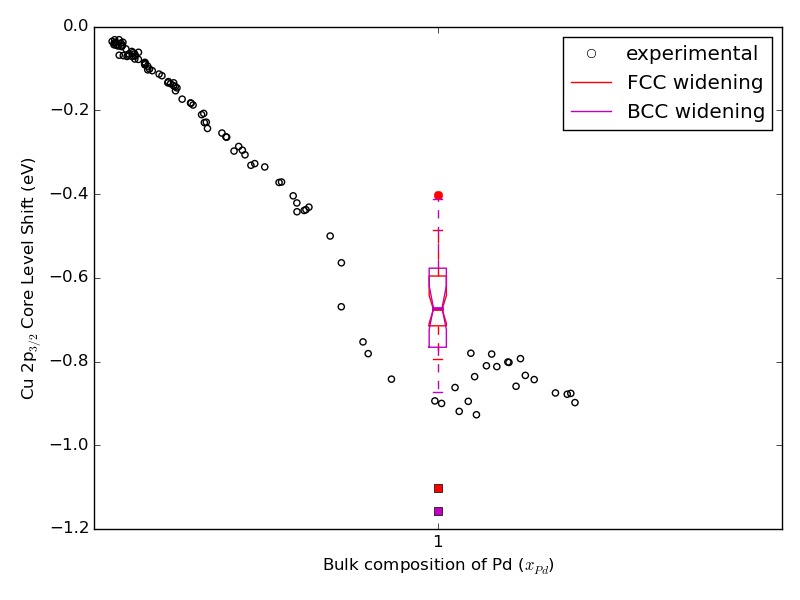
\includegraphics[width=4in]{./images/wid-compare.png}
\caption{\label{fig-wid-compare}Distinction between FCC (blue) and BCC (magenta) widening studies at 50 at.\% Pd. Results are compared with experimental data (black) and ground state configuration CLS (squares) for FCC and BCC structures. The ground state BCC structure is the B2 phase.}
\end{figure}

\begin{minted}[frame=lines,fontsize=\scriptsize,linenos]{python}
from ase.db import connect
import numpy as np
import matplotlib.pyplot as plt

# Import Gellman experimental data
d0x = np.array([entry[0] for entry in d0])
d0y = np.array([entry[1] for entry in d0])

# loads the ASE database and select certain keywords
db = connect('data.json')

keys = ['fcc', 'RN', '64atom']

CLSfcc = []
for k in db.select(keys + ['1cl', '0.50Cu-wid']):
    Cu0 = db.select(keys + ['0cl', '1.00Cu']).next().energy
    Cu1 = db.select(keys + ['1cl', '1.00Cu']).next().energy
    x0 = db.select(keys + ['0cl', '0.50Cu']).next().energy
    x1 = k.energy

    cls0 = x0 - Cu0
    cls1 = x1 - Cu1

    CLSfcc.append(cls1 - cls0)

CLSfcc = np.array(CLSfcc)

keys = ['bcc', 'RN', '64atom']

CLSbcc = []
for k in db.select(keys + ['1cl', '0.50Cu-wid']):
    Cu0 = db.select(keys + ['0cl', '1.00Cu']).next().energy
    Cu1 = db.select(keys + ['1cl', '1.00Cu']).next().energy
    x0 = db.select(keys + ['0cl', '0.50Cu']).next().energy
    x1 = k.energy

    cls0 = x0 - Cu0
    cls1 = x1 - Cu1

    CLSbcc.append(cls1 - cls0)

CLSbcc = np.array(CLSbcc)

keys = ['fcc', 'GS', '72atom']

Cu0 = db.select(keys + ['0cl', '1.00Cu']).next().energy
Cu1 = db.select(keys + ['1cl', '1.00Cu']).next().energy
x0 = db.select(keys + ['0cl', '0.50Cu']).next().energy
x1 = db.select(keys + ['1cl', '0.50Cu']).next().energy

cls0 = x0 - Cu0
cls1 = x1 - Cu1

CLSfgs = cls1 - cls0

keys = ['bcc', 'GS', '72atom', '1.00frac']

Cu0 = db.select(keys + ['0cl', '1.00Cu']).next().energy
Cu1 = db.select(keys + ['1cl', '1.00Cu']).next().energy
x0 = db.select(keys + ['0cl', '0.50Cu']).next().energy
x1 = db.select(keys + ['1cl', '0.50Cu']).next().energy

cls0 = x0 - Cu0
cls1 = x1 - Cu1

CLSbgs = cls1 - cls0

plt.figure()

plt.scatter(d0x, d0y, c='k', facecolor='none')
plt.plot(0.5, CLSfgs, marker='s', c='r')
plt.plot(0.5, CLSbgs, marker='s', c='m')
prox1 = plt.matplotlib.lines.Line2D([0],
                                    [0],
                                    linestyle="none",
                                    color='k',
                                    marker='o',
                                    mfc='none')

bp = plt.boxplot(CLSfcc,
                 notch=True,
                 positions=[0.5],
                 widths=[0.025],
                 sym='ro')

plt.setp(bp['boxes'], color='red')
plt.setp(bp['medians'], color='red', lw=2)
plt.setp(bp['fliers'], color='red')
plt.setp(bp['whiskers'], color='red')
plt.setp(bp['caps'], color='red')

prox2 = plt.matplotlib.lines.Line2D([0], [0], color='r')

bp = plt.boxplot(CLSbcc,
                 notch=True,
                 positions=[0.5],
                 widths=[0.025],
                 sym='mo')

plt.setp(bp['boxes'], color='m')
plt.setp(bp['medians'], color='m', lw=2)
plt.setp(bp['fliers'], color='m')
plt.setp(bp['whiskers'], color='m')
plt.setp(bp['caps'], color='m')

prox3 = plt.matplotlib.lines.Line2D([0], [0], color='m')

plt.xlabel('Bulk composition of Pd ($x_{Pd}$)')
plt.ylabel('Cu 2p$_{3/2}$ Core Level Shift (eV)')
plt.xlim(0, 1)
plt.ylim(-1.2, 0)
plt.legend([prox1, prox2, prox3],
           ['experimental', 'FCC widening', 'BCC widening'],
           numpoints=1, loc='best')
plt.tight_layout()

plt.savefig('./images/wid-compare.png')
\end{minted}

\section{Vegard's law for BCC CuPd}
\label{sec-8}
To simulate the 40 at. \% Pd environment of CuPd alloy, we must choose a normalized unit-cell volume that is representative of that composition. Volume is often shown to correlate linearly with the bulk composition of an alloy. We verify this computationally below by plotting the volumes of the ground state configurations of the BCC lattice against their compositions. These configurations are shown in Figure \ref{fig-vgd} plotted against a linear correlation between the normalized volumes of the pure component metals. The volumes of the ground state configurations are in good agreement with Vegard's law. Based on this result, we calculate the lattice constant of the 40 at.\% Pd structure using the linear relationship. The resulting normalized volume is shown by the red dot in Figure \ref{fig-vgd}.

\begin{figure}[H]
\centering
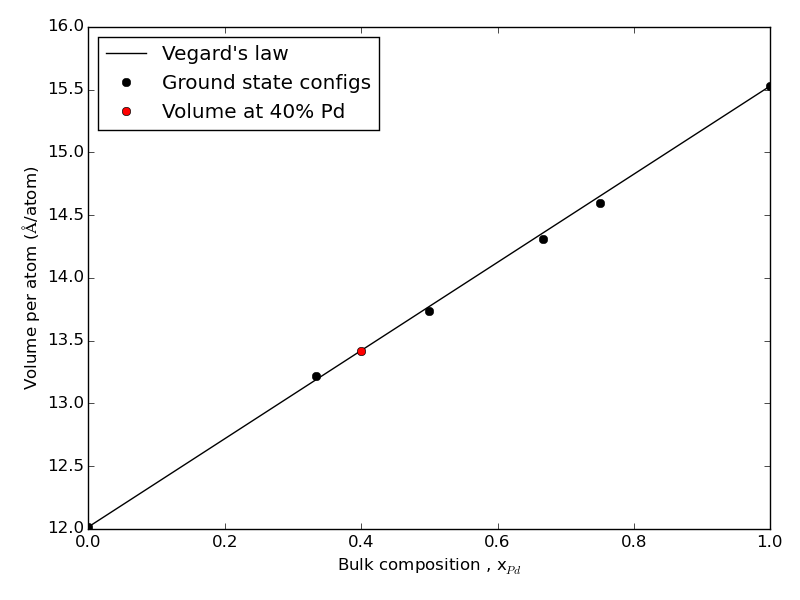
\includegraphics[width=4in]{./images/BCC-VGlaw.png}
\caption{\label{fig-vgd}Vegard's law compared with normalize volumes of ground state configurations for the BCC structure.}
\end{figure}

\begin{minted}[frame=lines,fontsize=\scriptsize,linenos]{python}
from ase.db import connect
import numpy as np
import matplotlib.pyplot as plt

# The ground state configurations
db = connect('data.json')

keys = ['bcc', 'GS', '72atom', '1.0frac', '0cl']

COMP, NORMV = [], []
for k in db.select(keys):

    volume = k.calculator_parameters.data.volume
    count = len(k.positions)

    COMP.append(1 - k.composition)
    NORMV.append(volume / count)

fit = np.poly1d(np.polyfit([min(COMP), max(COMP)],
                           [min(NORMV), max(NORMV)],
                           1))
X = np.linspace(0, 1)

# This is the lattice constant we expect for an alloy at 40 at.% Pd
c40 = (fit(0.4) * 2) ** (1./3)

print r"Vegard's law predicts 40 at.\% Pd to be {0:1.2f} Ang/atom".format(c40)

plt.figure()
plt.plot(X, fit(X), 'k-', label="Vegard's law")
plt.plot(COMP, NORMV, 'ko', label='Ground state configs')
plt.plot(0.4, fit(0.4), 'ro', label='Volume at 40% Pd')
plt.xlabel('Bulk composition , x$_{Pd}$')
plt.ylabel(r'Volume per atom ($\AA$/atom)')
plt.legend(loc='best', numpoints=1)
plt.tight_layout()
plt.savefig('./images/BCC-VGlaw.png')
\end{minted}

\section{Analysis of single impurity distance from excited atom in B2 phase}
\label{sec-9}
Here we analyze the effects of adding a single Cu impurity in the B2 structure on the CLS of a Cu atom. In a 54 atom super-cell there are four unique positions to place a Cu impurity relative to an excited Cu atom. Each of these positions represents a unique distance from the excited electron. Figure \ref{fig-imp} shows the resulting CLSs calculated for a B2 phase structure with a single Cu impurity at each of these four unique sites. As the Cu impurity gets closer to the excited electron, the CLS becomes increasingly positive. This effect is strongest at the first nearest neighbor to the excited Cu atom and drops off rapidly.

\begin{figure}[H]
\centering
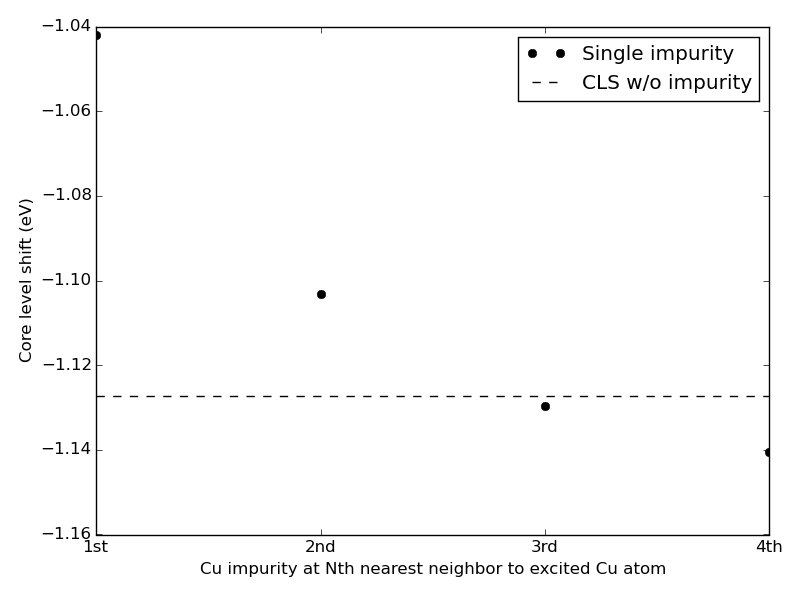
\includegraphics[width=4in]{./images/impurity.png}
\caption{\label{fig-imp}Effect on CLS of a single Cu impurity with distance from the excited atom in the B2 phase.}
\end{figure}

\begin{minted}[frame=lines,fontsize=\scriptsize,linenos]{python}
import matplotlib.pyplot as plt
from ase.db import connect

# loads the ASE database and select certain keywords
db = connect('data.json')

keys = ['bcc', 'GS', '54atom', '0.40lat', 'dis']

CLS, DIST = [], []
for k in db.select(keys + ['1cl']):
    dist = k.keywords[-1]

    Cu0 = db.select(['bcc', 'GS', '1.00frac', '0cl', '1.00Cu']).next().energy
    Cu1 = db.select(['bcc', 'GS', '1.00frac', '1cl', '1.00Cu']).next().energy
    x0 = db.select(keys + [dist, '0cl']).next().energy
    x1 = k.energy

    cls0 = x0 - Cu0
    cls1 = x1 - Cu1

    DIST.append(dist)
    CLS.append(cls1 - cls0)

plt.figure()
plt.plot(DIST[1:], CLS[1:], 'ko', label='Single impurity')
plt.plot([DIST[1], DIST[4]], [CLS[0], CLS[0]], 'k--', label='CLS w/o impurity')
plt.xlabel('Cu impurity at Nth nearest neighbor to excited Cu atom')
plt.ylabel('Core level shift (eV)')
plt.xticks([1, 2, 3, 4], ['1st', '2nd', '3rd', '4th'])
plt.legend(loc='best')
plt.tight_layout()
plt.savefig('./images/impurity.png')
\end{minted}

\section{Figures in the Manuscript}
\label{sec-10}
\subsection{Phase Diagram}
\label{sec-10-1}
This figure shows the EBSD data superimposed on the phase diagram, with the computational convex hull for the fcc and bcc lattices.

\begin{minted}[frame=lines,fontsize=\scriptsize,linenos]{python}
import matplotlib.pyplot as plt
import matplotlib.gridspec as gridspec
import matplotlib.image as mpimg
from matplotlib.offsetbox import OffsetImage, AnnotationBbox
from matplotlib.path import Path
import matplotlib.patches as patches
import numpy as np

# Import energies of FCC grounds states calculated by ATAT
d0x = np.array([entry[0] for entry in d0])
d0y = np.array([entry[1] for entry in d0])

# Import energies of BCC grounds states calculated by ATAT
d1x = np.array([entry[0] for entry in d1])
d1y = np.array([entry[1] for entry in d1])

# Removed the first composition since
# it is treated differently in the plot
g1 = np.array([0.2433, 0.3193, 0.3372, 0.3646, 0.3833,
               0.4219, 0.4519, 0.4725, 0.4829, 0.6920])

images = ['5.png', '24.png', '32.png', '34.png', '36.png',
          '38.png', '42.png', '45.png', '47.png', '48.png', '69.png']

mix0 = [d0x[2], d0x[2]]
mix1 = [d1x[1], d1x[1]]
mix2 = [d1x[2], d1x[2]]
mix3 = [d0x[5], d0x[5]]

zoom = 1.0  # Scales the size of the images
imageb = []
for img in images:

    # Make image into an array of colors
    image = mpimg.imread('images/{0}'.format(img))

    # Rescale each image based on zoom
    imageb.append(OffsetImage(image, zoom=zoom))


# BEGIN FIGURE
fig = plt.figure(figsize=(6, 5))

# Makes two subplots: ax0 - below, ax1 - above
gs0 = gridspec.GridSpec(1, 1, top=0.35, bottom=0.09,
                        right=0.98, left=0.1)
gs1 = gridspec.GridSpec(1, 1, top=0.98, bottom=0.37,
                        right=0.98, left=0.1, wspace=0.1)
ax0 = fig.add_subplot(gs0[0])
ax1 = fig.add_subplot(gs1[0])

# Plot the grounds state data for FCC and BCC
spl0, = ax0.plot(mix0, [0.001, d0y[2]], 'k--')
spl2, = ax0.plot(mix2, [0.001, d1y[2]], 'k--')
spl3, = ax0.plot(mix3, [0.001, d0y[5]], 'k--')

spl0.set_clip_on(False)
spl2.set_clip_on(False)
spl3.set_clip_on(False)

# Adding annotation
ax0.text(0.725, -1.0, 'BCC',
         size=12, color='g', weight='bold',
         horizontalalignment='left',
         verticalalignment='center')
ax0.text(0.725, -0.8, 'FCC',
         size=12, color='r', weight='bold',
         horizontalalignment='left',
         verticalalignment='center')

ax0.plot(d0x, d0y, 'r*-', label='FCC', zorder=5, ms=10)
ax0.plot(d1x, d1y, 'g*--', label='BCC', zorder=5, ms=10)

# Places an image on the plot at the xy coordinates.
arsty = 'arc,angleA=-90,armA=85'

ax1.text(0.785, 1130, 'at%', ha='center', size=10)

ax1.text(0.25, 1130, '5.0', ha='center', size=10)
ax1.add_artist(AnnotationBbox(imageb[0], xy=(0.25, 1020), pad=0))

del imageb[0]

for i, ib in enumerate(imageb):
    ax1.text(0.30 + 0.05*i, 1130,
             '{0:1.0f}'.format(g1[i]*100),
             ha='center',
             size=10)
    ax1.add_artist(AnnotationBbox(ib,
                                  xy=(g1[i], 800),
                                  xybox=(0.30 + 0.05*i, 1020),
                                  pad=0,
                                  arrowprops=dict(arrowstyle='->',
                                                  color='0.5',
                                                  zorder=5,
                                                  connectionstyle=arsty)
                                 )
                  )

ax1.scatter(g1, g1**0*800, c='r', marker='s', zorder=5, s=25)

# Plotting the fits
ax1.plot([0.2925, 0.345], [673.15, 673.15], 'k-', lw=2)

# Draw the Bezier curves used to estimate the phase boundries
verts = [[(0.4, 871.3), (0.31, 871.3), (0.3, 673.15), (0.3, 673.15)],
         [(0.4, 871.3), (0.36, 871.3), (0.346, 673.15), (0.346, 673.15)],
         [(0.2925, 673.15), (mix0[0], 500), (mix0[0], 0), (mix0[0], 0.0)],
         [(0.346, 673.15), (0.346, 500), (mix2[0], 400), (mix2[0], 0.0)],
         [(0.4, 871.3), (0.49, 871.3), (mix2[0], 0), (mix2[0], 0.0)],
         [(0.4, 871.3), (0.6, 871.3), (mix3[0], 0), (mix3[0], 0.0)]]

codes = [Path.MOVETO, Path.CURVE4, Path.CURVE4, Path.CURVE4]

for i, vert in enumerate(verts):
    path = Path(vert, codes)
    patch = patches.PathPatch(path, facecolor='none', lw=2)
    ax1.add_patch(patch)

# Plotting the predicting phase boundry at 0 K
ax1.scatter([mix0[0], mix2[0], mix3[0]],
            [0, 0, 0],
            c=['r', 'g', 'r'], marker='*',
            s=90, zorder=4)

# This code sets the zero line and then makes the dashed line a bit more solid
zero, = ax1.plot([0, 1], [0, 0], 'k--', lw=1.5)
dashes = [10, 10, 50, 10]  # 10 points on, 10 off, 50 on, 10 off
zero.set_dashes(dashes)

# Adding annotation to the phase regions
ax1.text((mix0[0] + mix2[0]) / 2.2, 300, 'mixed\nFCC/BCC',
         size=10,
         horizontalalignment='center',
         verticalalignment='center')
ax1.text((mix2[0] + mix3[0]) / 2.05, 300, 'mixed\nFCC/BCC',
         size=10,
         horizontalalignment='center',
         verticalalignment='center')
ax1.text((mix1[0] + mix2[0]) / 2.05, 670, 'B2',
         size=10,
         horizontalalignment='center',
         verticalalignment='center')

# Set parameters for each subplot
ax1.set_xlim(0.20, 0.80)
ax1.set_ylim(-10.0, 1200.0)
ax1.xaxis.tick_top()
ax1.tick_params(labeltop='off')
ax1.set_ylabel('Temperature (K)')
# Position the y-label properly
ax1.yaxis.set_label_coords(0.03, 0.7, transform=fig.transFigure)

ax0.set_xlim(0.20, 0.80)
ax0.set_ylim(-0.15, -0.02)
ax0.legend(loc='best', prop={'size': 10})
ax0.tick_params(labelleft='off')
# Position the y-label properly
ax0.yaxis.set_label_coords(0.06, 0.20, transform=fig.transFigure)
ax0.set_xlabel('Pd composition, $x$')  # label graph
ax0.set_ylabel('Formation\nenergy (a.u.)')

for ext in ['png', 'eps', 'pdf']:
    plt.savefig('../images/phase.{0}'.format(ext), dpi=300)

plt.show()
\end{minted}

\subsection{Experimental Data}
\label{sec-10-2}
This figure shows the anomalous CLS observed in this work, with comparisons to previous literature results (red triangles \cite{martensson-1981-elect-cu}, red squares \cite{cole-1997-deter-charg}).

\begin{minted}[frame=lines,fontsize=\scriptsize,linenos]{python}
import numpy as np
import matplotlib.pyplot as plt

# Import Gellman experimental data
d0x = np.array([entry[0] for entry in d0])
d0y = np.array([entry[1] for entry in d0])

# Import experimental data from reference 15
d1x = np.array([entry[0] for entry in d1])
d1y = np.array([entry[1] for entry in d1])

# Import experimental data from reference 5
d2x = np.array([entry[0] for entry in d2])
d2y = np.array([entry[1] for entry in d2])


# These phase boundries are read directly from the phase diagram
mix0 = 0.32790035
mix1 = 0.36635768
mix2 = 0.4411529

# This is the boundary we predict
mix3 = 0.55


# Create the figure
plt.figure(figsize=(6, 4))

# Plotting the data
plt.scatter(d0x, d0y, c='w', marker='s', s=25,
            label='This work')
plt.scatter(d1x, d1y, c='r', marker='^', s=25,
            label='Martensson et. al.')
plt.scatter(d2x, d2y, c='r', marker='D', s=25,
            label='Cole et. al.')

# Plotting the phase boundry lines
plt.plot([mix0, mix0], [-1.2, 0.0], 'k--')
plt.plot([mix1, mix1], [-1.2, 0.0], 'k-')
plt.plot([mix2, mix2], [-1.2, 0.0], 'k-')
plt.plot([mix3, mix3], [-1.2, 0.0], 'k--')

plt.xlabel('Pd composition, $x$')
plt.ylabel('Cu 2p$_{3/2}$ Core level shift (eV)')
plt.xlim(0, 1)
plt.ylim(-1.2, 0.0)
plt.legend(loc='best', scatterpoints=1, prop={'size': 10})
plt.tight_layout()

for ext in ['png', 'eps', 'pdf']:
    plt.savefig('../images/experiment.{0}'.format(ext), dpi=300)
\end{minted}

\subsection{He+ Sputtered Experimental Data}
\label{sec-10-3}
This figure illustrates that sputtered samples do not show the CLS anomaly, but annealed samples do show the anomaly.

\begin{minted}[frame=lines,fontsize=\scriptsize,linenos]{python}
import numpy as np
import matplotlib.pyplot as plt

# Import Gellman experimental data annealed at 800 K
d0x = np.array([entry[0] for entry in d0])
d0y = np.array([entry[1] for entry in d0])

# Import Gellman experimental data sputtered with He+
d1x = np.array([entry[0] for entry in d1])
d1y = np.array([entry[1] for entry in d1])


# These phase boundries are read directly from the phase diagram
mix0 = 0.32790035
mix1 = 0.36635768
mix2 = 0.4411529

# This is the boundary we predict
mix3 = 0.55


# Create the figure
plt.figure(figsize=(6, 4))

# Plotting the data
plt.scatter(d0x, d0y, c='w', marker='s', s=25)
plt.scatter(d1x, d1y, c='r', marker='s', s=25)

# Adding annotation
plt.text(0.56, -1.0, 'Annealed 800 K',
         size=12, color='k', weight='bold',
         horizontalalignment='left',
         verticalalignment='center')
plt.text(0.56, -0.55, 'He$^{+}$ Sputtered',
         size=12, color='r', weight='bold',
         horizontalalignment='left',
         verticalalignment='center')

plt.xlabel('Pd composition, $x$')
plt.ylabel('Cu 2p$_{3/2}$ Core level shift (eV)')
plt.xlim(0, 1)
plt.ylim(-1.2, 0.0)

plt.tight_layout()

for ext in ['png', 'eps', 'pdf']:
    plt.savefig('../images/sputtering.{0}'.format(ext), dpi=300)
\end{minted}

\subsection{Computational Comparison}
\label{sec-10-4}
This figure compares the CLSs measured in this work with previously computed CLS \cite{olovsson-2006-core-level}.

\begin{minted}[frame=lines,fontsize=\scriptsize,linenos]{python}
from ase.db import connect
import numpy as np
import matplotlib.pyplot as plt


# Import Gellman experimental data
d0x = np.array([entry[0] for entry in d0])
d0y = np.array([entry[1] for entry in d0])

# Import computational CS data from Olovsson et. al.
d1x = np.array([entry[0] for entry in d1])
d1y = np.array([entry[1] for entry in d1])


# loads the ASE database and select certain keywords
db = connect('data.json')

keys = ['fcc', 'RN', '64atom']

CLSfcc = []
for k in db.select(keys + ['1cl', '0.50Cu-wid']):
    Cu0 = db.select(keys + ['0cl', '1.00Cu']).next().energy
    Cu1 = db.select(keys + ['1cl', '1.00Cu']).next().energy
    x0 = db.select(keys + ['0cl', '0.50Cu']).next().energy
    x1 = k.energy

    cls0 = x0 - Cu0
    cls1 = x1 - Cu1

    CLSfcc.append(cls1 - cls0)

CLSfcc = np.array(CLSfcc)

keys = ['bcc', 'GS', '72atom', '1.00frac']

Cu0 = db.select(keys + ['0cl', '1.00Cu']).next().energy
Cu1 = db.select(keys + ['1cl', '1.00Cu']).next().energy
x0 = db.select(keys + ['0cl', '0.50Cu']).next().energy
x1 = db.select(keys + ['1cl', '0.50Cu']).next().energy

cls0 = x0 - Cu0
cls1 = x1 - Cu1

CLSbgs = cls1 - cls0

keys = ['fcc', 'GS', '72atom']

Cu0 = db.select(keys + ['0cl', '1.00Cu']).next().energy
Cu1 = db.select(keys + ['1cl', '1.00Cu']).next().energy
x0 = db.select(keys + ['0cl', '0.50Cu']).next().energy
x1 = db.select(keys + ['1cl', '0.50Cu']).next().energy

cls0 = x0 - Cu0
cls1 = x1 - Cu1

CLSfgs = cls1 - cls0

# Figure
# ------------------------------------------------------------------------
fig = plt.figure(figsize=(6, 4))
ax1 = fig.add_subplot(111)

ax1.scatter(d0x, d0y, c='w', marker='s', s=25,
            label='This work (expt.)')
ax1.scatter(d1x, d1y, c='r', marker='o', s=25,
            label='Olovsson et. al.')
ax1.scatter(0.5, CLSbgs, c='g', marker='*', s=90,
            label='This work (comp. B2)')
ax1.scatter(0.5, CLSfgs, c='r', marker='*', s=90,
            label='This work (comp. ordered FCC)')

ax1.legend(loc='best', scatterpoints=1, prop={'size': 10})


# These phase boundries are read directly from the phase diagram
mix0 = 0.32790035
mix1 = 0.36635768
mix2 = 0.4411529
mix3 = 0.55

# Plotting the phase boundry lines
plt.plot([mix0, mix0], [-1.2, 0.0], 'k--')
plt.plot([mix1, mix1], [-1.2, 0.0], 'k-')
plt.plot([mix2, mix2], [-1.2, 0.0], 'k-')
plt.plot([mix3, mix3], [-1.2, 0.0], 'k--')

ax1.set_xlabel('Pd composition, $x$')
ax1.set_ylabel('Cu 2p$_{3/2}$ Core Level Shift (eV)')

ax1.set_xlim(0, 1)
ax1.set_ylim(-1.2, 0.0)

ax2 = ax1.twiny()

bp = ax2.boxplot(CLSfcc,
                 notch=True,
                 positions=[0.5],
                 widths=[0.02],
                 sym='wo',
                 patch_artist=True)

for item in ['medians', 'fliers', 'whiskers', 'caps']:
    for obj in bp[item]:
        obj.set(color='r')

plt.tick_params(
    axis='x',          # changes apply to the x-axis
    which='both',      # both major and minor ticks are affected
    bottom='off',      # ticks along the bottom edge are off
    top='off',         # ticks along the top edge are off
    labeltop='off')    # labels along the bottom edge are off

plt.xlim(0, 1)
plt.ylim(-1.2, 0.0)

plt.tight_layout()

for ext in ['png', 'eps', 'pdf']:
    plt.savefig('../images/result.{0}'.format(ext), dpi=300)
\end{minted}

\subsection{Cu Impurities around excited fcc 50\% Pd ground state}
\label{sec-10-5}
This figure illustrates that adding excess Cu atoms compared to the stoichiometric number has a significant effect on the CLS of a Cu atom.

\begin{minted}[frame=lines,fontsize=\scriptsize,linenos]{python}
import matplotlib.pyplot as plt
from ase.db import connect
import matplotlib.gridspec as gridspec

# loads the ASE database and select certain keywords
db = connect('data.json')

keys = ['bcc', 'GS', '54atom', 'ensam']

CLS, IMP = [], []
for k in db.select(keys + ['1cl']):
    name = k.keywords[-2]

    Cu0 = db.select(['bcc', 'GS', '72atom', '0cl', '1.00Cu']).next().energy
    Cu1 = db.select(['bcc', 'GS', '72atom', '1cl', '1.00Cu']).next().energy
    x0 = db.select(keys + [name, '0cl']).next().energy
    x1 = k.energy

    cls0 = x0 - Cu0
    cls1 = x1 - Cu1

    IMP.append(int(name[1]))
    CLS.append(cls1 - cls0)

Cu0 = db.select(['bcc', 'GS', '72atom', '0cl', '1.00Cu']).next().energy
Cu1 = db.select(['bcc', 'GS', '72atom', '1cl', '1.00Cu']).next().energy

x0 = db.select(['bcc', 'GS', '54atom', '0cl', '1']).next().energy
x1 = db.select(['bcc', 'GS', '54atom', '1cl', '1']).next().energy

cls0 = x0 - Cu0
cls1 = x1 - Cu1

IMP.append(1)
CLS.append(cls1 - cls0)

Cu0 = db.select(['bcc', 'GS', '72atom', '0cl', '1.00Cu']).next().energy
Cu1 = db.select(['bcc', 'GS', '72atom', '1cl', '1.00Cu']).next().energy

x0 = db.select(['bcc', 'GS', '54atom', '0cl', '0']).next().energy
x1 = db.select(['bcc', 'GS', '54atom', '1cl', '0']).next().energy

cls0 = x0 - Cu0
cls1 = x1 - Cu1

IMP.append(0)
CLS.append(cls1 - cls0)

keys = ['fcc', 'GS', '54atom', 'ensam']

CLSf, IMPf = [], []
for k in db.select(keys + ['1cl']):
    name = k.keywords[-2]

    Cu0 = db.select(['bcc', 'GS', '72atom', '0cl', '1.00Cu']).next().energy
    Cu1 = db.select(['bcc', 'GS', '72atom', '1cl', '1.00Cu']).next().energy
    x0 = db.select(keys + [name, '0cl']).next().energy
    x1 = k.energy

    cls0 = x0 - Cu0
    cls1 = x1 - Cu1

    IMPf.append(int(name[1]))
    CLSf.append(cls1 - cls0)

fig = plt.figure()

gs0 = gridspec.GridSpec(1, 1, top=0.98, bottom=0.09,
                        right=0.52, left=0.1)
gs1 = gridspec.GridSpec(1, 1, top=0.98, bottom=0.09,
                        right=0.98, left=0.54, wspace=0.1)
ax1 = fig.add_subplot(gs0[0])
ax2 = fig.add_subplot(gs1[0])

ax1.scatter(IMP, CLS, c='g', marker='o', s=25)

# Adding annotation
ax1.text(0.15, -0.65, 'a) $x = 0.4$ BCC',
         size=16, weight='bold',
         horizontalalignment='left',
         verticalalignment='bottom')

ax1.set_ylim(-1.15, -0.6)
ax1.set_xlim(-0.1, 5.1)
ax1.set_ylabel('Cu 2p$_{3/2}$ Core Level Shift (eV)')


ax2.scatter(IMPf[0:], CLSf[0:], c='r', marker='o', s=25)


# Adding annotation
ax2.text(0.15, -0.65, 'b) $x = 0.5$ FCC',
         size=16, weight='bold',
         horizontalalignment='left',
         verticalalignment='bottom')


ax2.set_ylim(-1.15, -0.6)
ax2.set_xlim(-0.1, 5.1)
ax2.set_yticklabels([])

ax2.set_xlabel('Nearest-neighbor Cu atoms')
ax2.xaxis.set_label_coords(0.53, 0.04, transform=fig.transFigure)


for ext in ['png', 'eps', 'pdf']:
    plt.savefig('../images/impurity.{0}'.format(ext), dpi=300)
\end{minted}

\subsection{Strain Effects on CLS}
\label{sec-10-6}
Here we study the effect that strain has on CLS in the ordered B2 phase.

\begin{minted}[frame=lines,fontsize=\scriptsize,linenos]{python}
import matplotlib.pyplot as plt
import numpy as np
from ase.db import connect

db = connect('data.json')

# Import data for Vegard's Law
keys = ['bcc', 'GS', '72atom', '1.00frac', '0cl']

COMP, NORMV = [], []
for k in db.select(keys):

    volume = k.calculator_parameters.data.volume
    count = len(k.positions)

    COMP.append(1 - k.composition)
    NORMV.append(volume / count)

fit = np.poly1d(np.polyfit([min(COMP), max(COMP)],
                           [min(NORMV), max(NORMV)],
                           1))

keys = ['bcc', 'GS', '54atom']

CLS, NORMV = [], []
for k in db.select(keys + ['dis', '1cl', '0']):
    lat = k.keywords[-4]

    Cu0 = db.select(['bcc', 'GS', '72atom', '0cl', '1.00Cu']).next().energy
    Cu1 = db.select(['bcc', 'GS', '72atom', '1cl', '1.00Cu']).next().energy
    x0 = db.select(keys + [lat, 'dis', '0cl', '0']).next().energy
    x1 = k.energy

    cls0 = x0 - Cu0
    cls1 = x1 - Cu1

    CLS.append(cls1 - cls0)

    volume = k.calculator_parameters.data.volume
    count = len(k.positions)

    NORMV.append(volume / count)

fig = plt.figure(figsize=(3.25, 4))
ax1 = fig.add_subplot(111)

ax1.set_xlabel('Pd composition, $x$')
ax1.set_ylabel('Cu 2p$_{3/2}$ Core level shift (eV)')
ax1.set_xticks([0.3, 0.4, 0.5, 0.6])
ax1.set_xlim(0.3, 0.6)

ax2 = ax1.twiny()

ax2.set_xlabel(r'Volume per atom ($\AA^3$/atom)')
ax2.set_xlim(fit(0.3), fit(0.6))
ax2.set_xticks([13.1, 13.6, 14.1])

ax2.scatter([NORMV[0], NORMV[1], NORMV[2], NORMV[3]],
            [CLS[0], CLS[1], CLS[2], CLS[3]],
            c='g', marker='o', s=25)
ax2.scatter(NORMV[4], CLS[4],
            c='g', marker='*', s=90)

plt.tight_layout()

for ext in ['png', 'eps', 'pdf']:
    plt.savefig('../images/strain.{0}'.format(ext), dpi=300)
\end{minted}

\subsection{Abstract Figure}
\label{sec-10-7}

\begin{minted}[frame=lines,fontsize=\scriptsize,linenos]{python}
import numpy as np
import matplotlib.pyplot as plt

# Import Gellman experimental data
d0x = np.array([entry[0] for entry in d0])
d0y = np.array([entry[1] for entry in d0])


# Create the figure
plt.figure(figsize=(6, 4))

# Plotting the data
plt.scatter(d0x, d0y, c='w', marker='s', s=25)

# Plotting the phase boundry lines
plt.fill_between([d0x[74], d0x[86]], 0.0, -1.2, facecolor='blue', alpha=0.3)

plt.text(0.66, -1.0, 'Annealed 800 K',
         size=12, color='k', weight='bold',
         horizontalalignment='left',
         verticalalignment='center')

plt.text(d0x[74] + (d0x[86] - d0x[74]) / 2.0, -0.3, 'B2\nphase\npresent',
         size=12, color='k', weight='bold',
         horizontalalignment='center',
         verticalalignment='center')

plt.xlabel('Pd composition, $x$')
plt.ylabel('Cu 2p$_{3/2}$ Core level shift (eV)')
plt.xlim(0, 1)
plt.ylim(-1.2, 0.0)
plt.tight_layout()

for ext in ['png', 'eps', 'pdf']:
    plt.savefig('../images/abstract.{0}'.format(ext), dpi=100)
\end{minted}
\section{Tables}
\label{sec-11}
\begin{longtable}{rr}
\caption{\label{gellman}Experimental CLS data from the Gellman group}
\\
Pd composition & CLS (eV)\\
\hline
\endhead
\hline\multicolumn{2}{r}{Continued on next page} \\
\endfoot
\endlastfoot
0.0269813 & -0.035\\
0.0297052 & -0.043\\
0.0298903 & -0.039\\
0.0306752 & -0.031\\
0.0320379 & -0.037\\
0.0327642 & -0.044\\
0.0335744 & -0.043\\
0.0356661 & -0.046\\
0.0371202 & -0.031\\
0.0373192 & -0.068\\
0.0397335 & -0.039\\
0.0406291 & -0.047\\
0.0410614 & -0.047\\
0.0420247 & -0.044\\
0.0426483 & -0.037\\
0.0432437 & -0.069\\
0.0470047 & -0.053\\
0.0486784 & -0.071\\
0.0501848 & -0.068\\
0.0513886 & -0.065\\
0.0556464 & -0.059\\
0.0560298 & -0.071\\
0.0573344 & -0.062\\
0.0599001 & -0.065\\
0.0599441 & -0.077\\
0.0605434 & -0.070\\
0.0652239 & -0.078\\
0.0653107 & -0.061\\
0.0742488 & -0.088\\
0.0744329 & -0.091\\
0.0745899 & -0.085\\
0.0751520 & -0.087\\
0.0785503 & -0.094\\
0.0787241 & -0.103\\
0.0813005 & -0.101\\
0.0853100 & -0.105\\
0.0952431 & -0.113\\
0.0993672 & -0.117\\
0.1079250 & -0.134\\
0.1086790 & -0.131\\
0.1118760 & -0.136\\
0.1162570 & -0.141\\
0.1163720 & -0.134\\
0.1186510 & -0.143\\
0.1191040 & -0.153\\
0.1211770 & -0.146\\
0.1287410 & -0.173\\
0.1409070 & -0.182\\
0.1416260 & -0.183\\
0.1445900 & -0.187\\
0.1569620 & -0.210\\
0.1600410 & -0.207\\
0.1609820 & -0.229\\
0.1637550 & -0.228\\
0.1654820 & -0.243\\
0.1864910 & -0.254\\
0.1922910 & -0.263\\
0.1933480 & -0.264\\
0.2040620 & -0.297\\
0.2108350 & -0.286\\
0.2161710 & -0.295\\
0.2200070 & -0.306\\
0.2285980 & -0.331\\
0.2341590 & -0.327\\
0.2486840 & -0.335\\
0.2694640 & -0.372\\
0.2730900 & -0.371\\
0.2899790 & -0.404\\
0.2953090 & -0.421\\
0.2955210 & -0.442\\
0.3058850 & -0.439\\
0.3085280 & -0.437\\
0.3128480 & -0.431\\
0.3437190 & -0.500\\
0.3598750 & -0.669\\
0.3600180 & -0.564\\
0.3914210 & -0.753\\
0.3989420 & -0.781\\
0.4327220 & -0.842\\
0.4957900 & -0.894\\
0.5055460 & -0.900\\
0.5251070 & -0.862\\
0.5311500 & -0.919\\
0.5443070 & -0.895\\
0.5480690 & -0.780\\
0.5535330 & -0.836\\
0.5561730 & -0.927\\
0.5706780 & -0.810\\
0.5783010 & -0.782\\
0.5857750 & -0.812\\
0.6018300 & -0.801\\
0.6033790 & -0.802\\
0.6137170 & -0.859\\
0.6201390 & -0.793\\
0.6271850 & -0.833\\
0.6400550 & -0.843\\
0.6709160 & -0.875\\
0.6880810 & -0.878\\
0.6932410 & -0.876\\
0.6993090 & -0.898\\
\end{longtable}

\begin{longtable}{rr}
\caption{\label{gellman0}Experimental CLS data from the Gellman group annealed at 800 K}
\\
Pd composition & CLS (eV)\\
\hline
\endhead
\hline\multicolumn{2}{r}{Continued on next page} \\
\endfoot
\endlastfoot
0.970620 & -0.957\\
0.965044 & -0.966\\
0.963994 & -0.956\\
0.959141 & -0.953\\
0.955608 & -0.964\\
0.953451 & -0.948\\
0.952483 & -0.942\\
0.947701 & -0.957\\
0.947293 & -0.942\\
0.939694 & -0.914\\
0.929381 & -0.919\\
0.928183 & -0.936\\
0.909846 & -0.941\\
0.908060 & -0.896\\
0.885838 & -0.9\\
0.870965 & -0.887\\
0.837957 & -0.888\\
0.826530 & -0.889\\
0.826178 & -0.877\\
0.775287 & -0.859\\
0.761052 & -0.856\\
0.760694 & -0.869\\
0.759647 & -0.85\\
0.693820 & -0.821\\
0.688780 & -0.848\\
0.679913 & -0.819\\
0.619330 & -0.799\\
0.606321 & -0.805\\
0.591953 & -0.787\\
0.559281 & -0.759\\
0.551321 & -0.761\\
0.536408 & -0.733\\
0.535554 & -0.749\\
0.523631 & -0.737\\
0.518219 & -0.734\\
0.508245 & -0.847\\
0.499943 & -0.727\\
0.496518 & -0.727\\
0.494415 & -0.726\\
0.491134 & -0.724\\
0.486196 & -0.803\\
0.483744 & -0.847\\
0.481042 & -0.758\\
0.480636 & -0.804\\
0.479485 & -0.724\\
0.461502 & -0.842\\
0.460475 & -0.838\\
0.434494 & -0.792\\
0.424751 & -0.789\\
0.391747 & -0.73\\
0.386842 & -0.716\\
0.375641 & -0.636\\
0.361235 & -0.596\\
0.332138 & -0.501\\
0.315523 & -0.408\\
0.315459 & -0.447\\
0.295892 & -0.442\\
0.286464 & -0.406\\
0.260972 & -0.368\\
0.241481 & -0.359\\
0.236447 & -0.354\\
0.217134 & -0.321\\
0.201240 & -0.291\\
0.187263 & -0.266\\
0.180347 & -0.271\\
0.167832 & -0.23\\
0.147873 & -0.21\\
0.126934 & -0.169\\
0.117163 & -0.147\\
0.106729 & -0.146\\
0.084420 & -0.123\\
0.070176 & -0.092\\
0.056352 & -0.104\\
0.052974 & -0.102\\
0.042454 & -0.059\\
0.034982 & -0.073\\
0.027697 & -0.073\\
0.027649 & -0.041\\
0.019983 & -0.017\\
0.016671 & -0.024\\
0.012179 & -0.029\\
0.011053 & -0.027\\
0.010077 & -0.004\\
0.005538 & -0.005\\
0.003187 & 0.005\\
0.002711 & -0.001\\
0.002689 & 0.013\\
0.002680 & 0.013\\
0.002549 & -0.004\\
0.002514 & -0.001\\
0.002503 & 0.018\\
0.002453 & -0.002\\
0.002417 & 0.024\\
0.002398 & 0.017\\
0.002390 & 0.014\\
0.002370 & 0.007\\
0.002368 & -0.002\\
0.002332 & 0.02\\
0.002312 & 0.002\\
0.002241 & 0.003\\
0.002224 & 0.016\\
0.002204 & -0.008\\
0.002088 & 0.013\\
0.002082 & 0.019\\
0.001961 & 0.003\\
0.001957 & 0.014\\
0.001936 & 0.011\\
0.001930 & 0.005\\
0.001929 & 0.004\\
0.001634 & 0.001\\
0.001569 & 0.011\\
0.001508 & 0\\
\end{longtable}

\begin{longtable}{rr}
\caption{\label{gellman1}Experimental CLS data from the Gellman group annealed at 800 K and sputtered with He+}
\\
Pd composition & CLS (eV)\\
\hline
\endhead
\hline\multicolumn{2}{r}{Continued on next page} \\
\endfoot
\endlastfoot
0.970010 & -0.868\\
0.963072 & 0.112\\
0.958901 & 0.119\\
0.948199 & -0.936\\
0.934726 & -0.917\\
0.920189 & -0.849\\
0.904226 & -0.873\\
0.902070 & 0.112\\
0.878280 & 0.285\\
0.873952 & -0.82\\
0.860939 & -0.711\\
0.855476 & -0.851\\
0.796308 & -0.757\\
0.779666 & 0.284\\
0.777827 & -0.803\\
0.739604 & -0.815\\
0.707311 & -0.763\\
0.683702 & -0.794\\
0.670810 & -0.72\\
0.659100 & -0.76\\
0.635587 & -0.719\\
0.625711 & -0.725\\
0.589491 & -0.643\\
0.587265 & 0.111\\
0.582688 & -0.735\\
0.574745 & -0.718\\
0.572542 & -0.667\\
0.541924 & -0.669\\
0.533617 & -0.734\\
0.517108 & -0.665\\
0.512565 & -0.66\\
0.479262 & -0.659\\
0.469572 & -0.69\\
0.468380 & -0.678\\
0.467112 & -0.721\\
0.464322 & -0.712\\
0.460976 & -0.676\\
0.458345 & -0.701\\
0.427268 & -0.625\\
0.411424 & -0.674\\
0.408883 & -0.704\\
0.398039 & -0.614\\
0.389279 & -0.623\\
0.368202 & -0.528\\
0.362499 & -0.592\\
0.320597 & -0.519\\
0.315641 & -0.489\\
0.313963 & -0.489\\
0.286363 & -0.418\\
0.276247 & -0.38\\
0.268089 & -0.357\\
0.264348 & -0.444\\
0.243958 & -0.367\\
0.240136 & -0.303\\
0.227346 & -0.344\\
0.218997 & -0.33\\
0.205084 & -0.278\\
0.190394 & -0.289\\
0.187310 & -0.217\\
0.181756 & -0.23\\
0.174281 & -0.245\\
0.163896 & -0.224\\
0.153409 & -0.255\\
0.148057 & -0.177\\
0.145305 & -0.19\\
0.130202 & -0.173\\
0.120032 & -0.137\\
0.115373 & -0.151\\
0.112777 & -0.176\\
0.101079 & -0.114\\
0.090852 & -0.143\\
0.079278 & -0.094\\
0.076086 & -0.137\\
0.070458 & -0.095\\
0.064294 & -0.097\\
0.052721 & -0.057\\
0.051671 & -0.069\\
0.043731 & -0.067\\
0.039242 & -0.021\\
0.037079 & -0.043\\
0.035688 & -0.027\\
0.030497 & -0.023\\
0.026987 & -0.047\\
0.020494 & -0.006\\
0.018899 & -0.047\\
0.014944 & 0.007\\
0.012090 & 0.001\\
0.010152 & -0.006\\
0.009648 & 0.006\\
0.009396 & 0.002\\
0.009141 & 0.002\\
0.009062 & -0.001\\
0.008566 & 0.029\\
0.008015 & -0.002\\
0.007929 & -0.014\\
0.007349 & 0.001\\
0.007300 & 0.004\\
0.007010 & -0.002\\
0.006850 & -0.017\\
0.006839 & -0.008\\
0.006726 & 0.002\\
0.006706 & 0.014\\
0.006656 & -0.001\\
0.006598 & -0.021\\
0.006523 & -0.011\\
0.006378 & -0.007\\
0.006197 & -0.004\\
0.006100 & 0.002\\
0.006076 & 0.008\\
0.006071 & 0\\
0.006053 & -0.016\\
0.006047 & -0.001\\
0.006030 & 0.033\\
0.005964 & -0.004\\
0.005942 & -0.013\\
0.005930 & -0.025\\
0.005911 & -0.004\\
0.005907 & -0.018\\
0.005827 & -0.027\\
0.005618 & -0.001\\
0.005575 & 0.002\\
0.005545 & 0.019\\
0.005545 & -0.024\\
0.005267 & -0.009\\
0.004978 & 0.004\\
0.004831 & -0.008\\
0.004178 & -0.003\\
0.003656 & 0\\
\end{longtable}


\begin{table}[H]
\caption{\label{ref-15}Experimental CLS data read from figure \cite{martensson-1981-elect-cu}}
\centering
\begin{tabular}{rr}
Pd composition & CLS (eV)\\
\hline
0.000 & 0.0\\
0.067 & -0.025\\
0.166 & -0.063\\
0.262 & -0.212\\
0.250 & -0.244\\
0.290 & -0.298\\
0.387 & -0.400\\
0.433 & -0.453\\
0.400 & -0.482\\
0.450 & -0.475\\
0.500 & -0.588\\
0.650 & -0.698\\
0.670 & -0.748\\
0.780 & -0.837\\
0.826 & -0.868\\
0.946 & -0.976\\
\end{tabular}
\end{table}

\begin{table}[H]
\caption{\label{ref-5}Experimental CLS data read from figure \cite{cole-1997-deter-charg}}
\centering
\begin{tabular}{rr}
Pd composition & CLS (eV)\\
\hline
0.2 & -0.25\\
0.5 & -0.70\\
\end{tabular}
\end{table}

\begin{table}[H]
\caption{\label{bcc}BCC Cluster expansion ground states}
\centering
\begin{tabular}{rrrr}
Pd comp. & Normalized energy (eV/atom) & Energy (eV/atom) & ATAT Structure\\
\hline
0.000000 & 0.030315 & 0.031500 & 0\\
0.333333 & -0.115639 & -0.115863 & 131\\
0.500000 & -0.127902 & -0.127745 & 3\\
0.666667 & -0.085447 & -0.083958 & 7\\
0.750000 & -0.061554 & -0.061584 & 15\\
1.000000 & 0.040240 & 0.040956 & 1\\
\end{tabular}
\end{table}

\begin{table}[H]
\caption{\label{fcc}FCC Cluster expansion ground states}
\centering
\begin{tabular}{rrrr}
Pd comp. & Normalized energy (eV/atom) & Energy (eV/atom) & ATAT Structure\\
\hline
0.000000 & 0.000000 & 0.010429 & 0\\
0.125000 & -0.054559 & -0.049823 & 470\\
0.250000 & -0.104835 & -0.103771 & 27\\
0.375000 & -0.117808 & -0.113541 & 455\\
0.500000 & -0.117016 & -0.114034 & 3\\
0.625000 & -0.097850 & -0.094601 & 625\\
0.750000 & -0.073519 & -0.066942 & 28\\
0.833333 & -0.052152 & -0.046461 & 80\\
1.000000 & 0.000000 & 0.001212 & 1\\
\end{tabular}
\end{table}

\begin{table}[H]
\caption{\label{cs-method}Computational CLS data read from figure in \cite{olovsson-2002-core-level} using CS method}
\centering
\begin{tabular}{rr}
Pd composition & CLS (eV)\\
\hline
0.15 & -0.243\\
0.2 & -0.314\\
0.25 & -0.382\\
0.3 & -0.471\\
0.4 & -0.626\\
0.5 & -0.773\\
0.6 & -0.878\\
0.7 & -0.986\\
0.75 & -1.015\\
0.8 & -1.063\\
0.9 & -1.142\\
\end{tabular}
\end{table}

\begin{table}[H]
\caption{\label{is-method}Computational CLS data read from figure in \cite{olovsson-2002-core-level} using IS method.}
\centering
\begin{tabular}{rr}
Pd composition & CLS (eV)\\
\hline
0.1 & -0.162\\
0.15 & -0.243\\
0.2 & -0.328\\
0.25 & -0.395\\
0.3 & -0.491\\
0.4 & -0.654\\
0.5 & -0.789\\
0.53 & -0.821\\
0.6 & -0.894\\
0.7 & -0.989\\
0.75 & -1.031\\
0.77 & -1.047\\
0.8 & -1.069\\
0.9 & -1.145\\
\end{tabular}
\end{table}

\bibliographystyle{elsarticle-num}
\bibliography{/Users/jkitchin/Desktop/cappa/kitchingroup-51/supporting-information/supporting-information}
% Emacs 25.1.50.1 (Org mode 8.2.10)
\end{document}